% This must be in the first 5 lines to tell arXiv to use pdfLaTeX, which is strongly recommended.
\pdfoutput=1
% In particular, the hyperref package requires pdfLaTeX in order to break URLs across lines.

\documentclass[11pt]{article}
% \usepackage{showframe}
% Change "review" to "final" to generate the final (sometimes called camera-ready) version.
% Change to "preprint" to generate a non-anonymous version with page numbers.
\usepackage[preprint]{acl}

% Standard package includes
\usepackage{times}
\usepackage{latexsym}

% For proper rendering and hyphenation of words containing Latin characters (including in bib files)
\usepackage[T1]{fontenc}
% For Vietnamese characters
% \usepackage[T5]{fontenc}
% See https://www.latex-project.org/help/documentation/encguide.pdf for other character sets

% This assumes your files are encoded as UTF8
\usepackage[utf8]{inputenc}

% This is not strictly necessary, and may be commented out,
% but it will improve the layout of the manuscript,
% and will typically save some space.
\usepackage{microtype}

% This is also not strictly necessary, and may be commented out.
% However, it will improve the aesthetics of text in
% the typewriter font.
\usepackage{inconsolata}

% Including images in your LaTeX document requires adding
% additional package(s)
\usepackage{graphicx}

% Our LaTeX packages
\usepackage{array}
\usepackage{amsfonts}
\usepackage{amsmath}
\usepackage{booktabs}
\usepackage{xspace}
\usepackage{paralist}
\usepackage{algorithm}
\usepackage{colortbl}
\usepackage[noend]{algpseudocode}
\usepackage{multirow}
\usepackage{cuted}
\usepackage{tcolorbox}
\usepackage{caption}
\tcbuselibrary{breakable}  % Load the breakable library
\usepackage{multicol}
% \usepackage[table]{xcolor}
% \usepackage{wasysym} % for \twonote

\definecolor{customGreen}{RGB}{223, 242, 223}
\definecolor{customYellow}{RGB}{250, 249, 214}
\definecolor{customRed}{RGB}{242, 223, 223}
\definecolor{customBlue}{RGB}{214, 224, 250}

\newtcolorbox[list inside=prompt,auto counter,number within=section]{prompt}[1][]{
    colbacktitle=black!60,
    coltitle=white,
    fontupper=\footnotesize,
    boxsep=5pt,
    left=0pt,
    right=0pt,
    top=0pt,
    bottom=0pt,
    boxrule=1pt,
    title={#1},
    breakable,
    #1, % Additional options
}

% If the title and author information does not fit in the area allocated, uncomment the following
%
%\setlength\titlebox{<dim>}
%
% and set <dim> to something 5cm or larger.

% Our LaTeX commands
\newcolumntype{L}[1]{>{\raggedright\let\newline\\\arraybackslash\hspace{0pt}}m{#1}}
\newcolumntype{C}[1]{>{\centering\let\newline\\\arraybackslash\hspace{0pt}}m{#1}}
\newcolumntype{R}[1]{>{\raggedleft\let\newline\\\arraybackslash\hspace{0pt}}m{#1}}

\DeclareMathOperator*{\argmax}{\arg\max}
\newcommand{\zhili}[1]{\textcolor{blue}{(Zhili: #1)}}
\newcommand{\chenxin}[1]{\textcolor{red}{(Chenxin: #1)}}
\newcommand{\pavlos}[1]{\textcolor{orange}{(Pavlos: #1)}}
\newcommand{\pascual}[1]{\textcolor{brown}{(Pascual: #1)}}
\newcommand{\gear}{\textsc{GeAR}\xspace}

\title{\gear: Graph-enhanced Agent for Retrieval-augmented Generation}

\author{{\bf Zhili Shen}$^{\mathbf{\dagger}}$ \quad {\bf Chenxin Diao}$^{\mathbf{\dagger}}$ \quad {\bf Pavlos Vougiouklis}$^{\mathbf{\dagger}}$ \quad {\bf Pascual Merita}$^{\mathbf{\dagger}}$ \\
{\bf Shriram Piramanayagam} \quad {\bf Damien Graux} \quad {\bf Dandan Tu}\\ {\bf Zeren Jiang} \quad {\bf Ruofei Lai} \quad {\bf Yang Ren} \quad \quad {\bf Jeff Z. Pan}\\ 
Huawei Technologies Co., Ltd.
\\Edinburgh, United Kingdom\\\texttt{\{}{\href{mailto:zhilishen@huawei.com}{\texttt{zhilishen}}}\texttt{,} 
\href{mailto:chenxindiao@huawei.com}{\texttt{chenxindiao}}\texttt{,} \href{mailto:pavlos.vougiouklis@huawei.com}{\texttt{pavlos.vougiouklis}}\texttt{,}
\href{mailto:pascual.merita@h-partners.com}{\texttt{pascual.merita}}\texttt{\}@huawei.com}\\\texttt{\{}{\href{mailto:renyang1@huawei.com}{\texttt{renyang1}}}\texttt{,} 
\href{mailto:jeff.pan@huawei.com}{\texttt{jeff.pan}}\texttt{\}@huawei.com}\\
}


\begin{document}
\maketitle
\begin{abstract}
Retrieval-augmented generation systems rely on effective document retrieval capabilities. By design, conventional sparse or dense retrievers face challenges in multi-hop retrieval scenarios. In this paper, we present \gear, which advances RAG performance through two key innovations: \begin{inparaenum}[(i)] \item graph expansion, which enhances any conventional base retriever, such as BM25, and \item an agent framework that incorporates graph expansion\end{inparaenum}. Our evaluation demonstrates \gear 's superior retrieval performance on three multi-hop question answering datasets. Additionally, our system achieves state-of-the-art results with improvements exceeding $10\%$ on the challenging MuSiQue dataset, while requiring fewer tokens and iterations compared to other multi-step retrieval systems.  
\end{abstract}
\renewcommand{\thefootnote}
{\fnsymbol{footnote}}
\setcounter{footnote}{2}
\footnotetext{The authors contributed equally to this work.}
\renewcommand{\thefootnote}
{\arabic{footnote}}
\setcounter{footnote}{0}

\documentclass[11pt]{report}
\usepackage[margin=2cm]{geometry}
\usepackage{graphicx}
\usepackage{float}
\usepackage{times}
\usepackage{url}
\usepackage[dvipsnames]{xcolor}
\usepackage{hyperref}

\newcommand{\specialcell}[2][c]{\begin{tabular}[#1]{@{}c@{}}#2\end{tabular}}

\newcommand{\Gap}{\texorpdfstring{\hfill}{}}
\newcommand{\Rec}{\texorpdfstring{{\small\emph{\color{ccai-blue}{\fbox{High Leverage}}}}}{}}
\newcommand{\HighRisk}{\texorpdfstring{{\small\emph{\color{ccai-yellow-darker}{\fbox{Uncertain Impact}}}}}{}}
\newcommand{\Longterm}{\texorpdfstring{{\small\emph{\color{ccai-green}{\fbox{Long-term}}}}}{}}

\begin{document}

\begin{abstract}
Climate change is one of the greatest challenges facing humanity, and we, as machine learning experts, may wonder how we can help. Here we describe how machine learning can be a powerful tool in reducing greenhouse gas emissions and helping society adapt to a changing climate. From smart grids to disaster management, we identify high impact problems where existing gaps can be filled by machine learning, in collaboration with other fields. Our recommendations encompass exciting research questions as well as promising business opportunities. We call on the machine learning community to join the global effort against climate change.
\vskip .5in
\end{abstract}

\part*{Introduction}
The effects of climate change are increasingly visible.\footnote{For a layman's introduction to the topic of climate change, see \cite{romm2018climate, archer2010climate}.} Storms, droughts, fires, and flooding have become stronger and more frequent \cite{field2012managing}. Global ecosystems are changing, including the natural resources and agriculture on which humanity depends. The 2018 intergovernmental report on climate change estimated that the world will face catastrophic consequences unless global greenhouse gas emissions are eliminated within thirty years \cite{ipcc_global_2018}. Yet year after year, these emissions rise.

Addressing climate change involves mitigation (reducing emissions) and adaptation (preparing for unavoidable consequences). Both are multifaceted issues. Mitigation of greenhouse gas (GHG) emissions requires changes to electricity systems, transportation, buildings, industry, and land use. Adaptation requires planning for resilience and disaster management, given an understanding of climate and extreme events. Such a diversity of problems can be seen as an opportunity: there are many ways to have an impact.

In recent years, machine learning (ML) has been recognized as a broadly powerful tool for technological progress. Despite the growth of movements applying ML and AI to problems of societal and global good,\footnote{See the AI for social good movement (e.g.~\cite{hager2019artificial, berendt2019ai}), ML for the developing world~\cite{de2018machine}, the computational sustainability movement (e.g.~\cite{kelling2018computational, joppa2017case, lassig2016computational, gomes2009computational, dietterich2009machine}, the American Meteorological Society's Committee on AI Applications to Environmental Science, and the field of Climate Informatics (\url{www.climateinformatics.org}) \cite{Monteleoni2013chapter}, as well as the relevant survey papers \cite{faghmous2014big, kaack2019challenges, ford2016opinion}.} there remains the need for a concerted effort to identify how these tools may best be applied to tackle climate change. Many ML practitioners wish to act, but are uncertain how. On the other side, many fields have begun actively seeking input from the ML community.

This paper aims to provide an overview of where machine learning can be applied with high impact in the fight against climate change, through either effective engineering or innovative research. The strategies we highlight include climate mitigation and adaptation, as well as meta-level tools that enable other strategies. In order to maximize the relevance of our recommendations, we have consulted experts across many fields (see \hyperref[sec:acknowledgments]{{\small{Acknowledgments}}}) in the preparation of this paper.


\begin{table}
\begin{small}
\begin{center}
\begin{tabular}{l l l l l l l l l l l l}  \toprule
     \multicolumn{2}{l}{ }
         & \small{\rotatebox{90}{\parbox{2.2cm}{Causal\\inference}}}
         & \small{\rotatebox{90}{\parbox{2.2cm}{Computer\\vision}}}
         & \small{\rotatebox{90}{\parbox{2.2cm}{Interpretable\\models}}}
         & \small{\rotatebox{90}{NLP}}
         & \small{\rotatebox{90}{\parbox{2.2cm}{RL \& Control}}}
        %  & \small{\rotatebox{90}{Robotics}}
         & \small{\rotatebox{90}{\parbox{2.2cm}{Time-series analysis}}}
         & \small{\rotatebox{90}{\parbox{2.2cm}{Transfer\\learning}}}
         & \small{\rotatebox{90}{\parbox{2.2cm}{Uncertainty\\quantification}}}
         & \small{\rotatebox{90}{\parbox{2.2cm}{Unsupervised\\learning}}}
    \\ \midrule
    \rowcolor{ccai-blue-lightest}
    \multicolumn{2}{l}{1 \hyperref[sec:electricity-systems]{Electricity systems}} 
        & % Causal inf
        &  % Comp vision
        & % Interpretable ml
        & % nlp
        & % rl + control
        & % time series
        & % transfer
        & % UQ
        & \\% unsupervised \ref{sub
    & \hyperref[sec:electricity-lowCarbon]{Enabling low-carbon electricity}
        & % Causal inf
        & $\bullet$% Comp vision
        & $\bullet$% % Interpretable ml
        & % % nlp
        & $\bullet$%% rl + control
        & $\bullet$% % time series
        & % transfer
        & $\bullet$% % UQ
        & $\bullet$\\% unsupervised 
    & \hyperref[sec:electricity-currentSystemImpact]{Reducing current-system impacts}
        & % Causal inf
        & $\bullet$% Comp vision
        & % Interpretable ml
        & % nlp
        & % rl + control
        & $\bullet$% % time series
        & % transfer
        & $\bullet$% % UQ
        & $\bullet$\\% unsupervised 
    & \hyperref[sec:electricity-developing]{Ensuring global impact}
        & % Causal inf
        & $\bullet$% Comp vision
        & % Interpretable ml
        & % nlp
        & % rl + control
        & % time series
        & $\bullet$ % transfer
        & % UQ
        & $\bullet$\\% unsupervised 
    \rowcolor{ccai-blue-lightest}
    \multicolumn{2}{l}{2 \hyperref[sec:transportation]{Transportation}} 
        & % Causal inf
        & % Comp vision
        &% Interpretable ml
        & % nlp
        & % rl + control
        & % time series
        & % transfer
        & % UQ
        & \\% unsupervised 
    & \hyperref[sec:TReducing]{Reducing transport activity}
        & % Causal inf
        & $\bullet$% Comp vision
        & % Interpretable ml
        & % nlp
        & % rl + control
        & $\bullet$% time series
        & % transfer
        & $\bullet$% UQ
        & $\bullet$\\% unsupervised     
   & \hyperref[sec:TEfficient]{Improving vehicle efficiency}
        & % Causal inf
        & $\bullet$% Comp vision
        & % Interpretable ml
        & % nlp
        & $\bullet$% rl + control
        & % time series
        & % transfer
        & % UQ
        & \\% unsupervised    
   & \hyperref[sec:TFuels]{Alternative fuels \& electrification}
        & % Causal inf
        & % Comp vision
        & % Interpretable ml
        & % nlp
        & $\bullet$% rl + control
        & % time series
        & % transfer
        & % UQ
        & $\bullet$ \\% unsupervised    
   & \hyperref[sec:modalshift]{Modal shift}
        & $\bullet$% Causal inf
        & $\bullet$% Comp vision
        & % Interpretable ml
        & % nlp
        & % rl + control
        & $\bullet$% time series
        & % transfer
        & $\bullet$% UQ
        & \\% unsupervised    
    \rowcolor{ccai-blue-lightest}
    \multicolumn{2}{l}{3 \hyperref[sec:buildings-cities]{Buildings and cities}} 
        & % Causal inf
        & % Comp vision
        & % Interpretable ml
        & % nlp
        & % rl + control
        & % time series
        & % transfer
        & % UQ
        & \\% unsupervised 
    & \hyperref[sec:indv]{Optimizing buildings}
        & $\bullet$% Causal inf
        & % Comp vision
        & % Interpretable ml
        & % nlp
        & $\bullet$% rl + control
        & $\bullet$% time series
        & $\bullet$% transfer
        & % UQ
        & \\% unsupervised 
    & \hyperref[sec:distr]{Urban planning}
        & % Causal inf
        & $\bullet$% Comp vision
        & % Interpretable ml
        & % nlp
        & % rl + control
        & $\bullet$% time series
        & $\bullet$% transfer
        & % UQ
        & $\bullet$\\% unsupervised 
    & \hyperref[sec:cities]{The future of cities}
        & % Causal inf
        & % Comp vision
        & % Interpretable ml
        & $\bullet$%% nlp
        & % rl + control
        & %% time series
        & $\bullet$%% transfer
        & $\bullet$% UQ
        & $\bullet$\\% unsupervised 
    \rowcolor{ccai-blue-lightest}
    \multicolumn{2}{l}{4 \hyperref[sec:industry]{Industry}} 
        & % Causal inf
        & % Comp vision
        & % Interpretable ml
        & % nlp
        & % rl + control
        & % time series
        & % transfer
        & % UQ
        & \\% unsupervised 
    & \hyperref[sec:supplychains]{Optimizing supply chains}
        & % Causal inf
        & $\bullet$ %% Comp vision
        & % Interpretable ml
        & % nlp
        & $\bullet$ % rl + control
        & $\bullet$ % time series
        & % transfer
        & % UQ
        & \\% unsupervised 
    & \hyperref[sec:materialsandconstruction]{Improving materials}
        & %% Causal inf
        & % Comp vision
        & % Interpretable ml
        & % nlp
        & % rl + control
        & % time series
        & %% transfer
        & % UQ
        & $\bullet$ \\% unsupervised 
    & \hyperref[sec:demandresponse]{Production \& energy}
        & %% Causal inf
        & $\bullet$%% Comp vision
        & $\bullet$ %% Interpretable ml
        & % nlp
        & $\bullet$% rl + control
        & %% time series
        & %% transfer
        & % UQ
        & \\% unsupervised 
    \rowcolor{ccai-blue-lightest}
    \multicolumn{2}{l}{5 \hyperref[sec:afolu]{Farms \& forests}} 
        & % Causal inf
        & % Comp vision
        & % Interpretable ml
        & % nlp
        & % rl + control
        & % time series
        & % transfer
        & % UQ
        & \\% unsupervised 
    & \hyperref[sec:emissions-detection]{Remote sensing of emissions}
        & % Causal inf
        & $\bullet$% Comp vision
        & % Interpretable ml
        & % nlp
        & % rl + control
        & % time series
        & % transfer
        & % UQ
        & \\% unsupervised 
    & \hyperref[sec:agriculture]{Precision agriculture}
        & % Causal inf
        & $\bullet$% Comp vision
        & % Interpretable ml
        & % nlp
        & $\bullet$% rl + control
        & $\bullet$% time series
        & % transfer
        & % UQ
        & \\% unsupervised 
    & \hyperref[sec:peatlands]{Monitoring peatlands}
        & % Causal inf
        & $\bullet$% Comp vision
        & % Interpretable ml
        & % nlp
        & % rl + control
        & % time series
        & % transfer
        & % UQ
        & \\% unsupervised 
    & \hyperref[sec:forests]{Managing forests}
        & % Causal inf
        & $\bullet$% Comp vision
        & % Interpretable ml
        & % nlp
        & $\bullet$ % rl + control
        & $\bullet$ % time series
        & % transfer
        & % UQ
        & \\% unsupervised 
    \rowcolor{ccai-blue-lightest}
    \multicolumn{2}{l}{6 \hyperref[sec:ccs]{Carbon dioxide removal}}
        & % Causal inf
        & % Comp vision
        & % Interpretable ml
        & % nlp
        & % rl + control
        & % time series
        & % transfer
        & % UQ
        & \\
    & \hyperref[sec:ccs]{Direct air capture}
        & % Causal inf
        & % Comp vision
        & % Interpretable ml
        & % nlp
        & % rl + control
        & % time series
        & % transfer
        & % UQ
        & $\bullet$\\% unsupervised 
    & \hyperref[subsubsec: sequestrativervin]{Sequestering~\cd}
        & % Causal inf
        & $\bullet$% Comp vision
        & % Interpretable ml
        & % nlp
        & % rl + control
        & % time series
        & % transfer
        & $\bullet$% UQ
        & $\bullet$\\% unsupervised 
    \rowcolor{ccai-blue-lightest}
    \multicolumn{2}{l}{7 \hyperref[sec: climate prediction]{Climate prediction}} 
        & % Causal inf
        & % Comp vision
        & % Interpretable ml
        & % nlp
        & % rl + control
        & % time series
        & % transfer
        & % UQ
        & \\% unsupervised 
    & \hyperref[sec:climate-models-params]{Uniting data, ML \& climate science}
        & % Causal inf
        & $\bullet$% Comp vision
        & $\bullet$% Interpretable ml
        & % nlp
        & % rl + control
        & $\bullet$% time series
        & % transfer
        & $\bullet$% UQ
        & \\% unsupervised 
    & \hyperref[sec:models-extreme-events]{Forecasting extreme events}
        & % Causal inf
        & $\bullet$% Comp vision
        & $\bullet$% Interpretable ml
        & % nlp
        & % rl + control
        & $\bullet$% time series
        & % transfer
        & $\bullet$% UQ
        & \\% unsupervised 
    \rowcolor{ccai-blue-lightest}
    \multicolumn{2}{l}{8 \hyperref[sec:societal-impacts]{Societal impacts}} 
        & % Causal inf
        & % Comp vision
        & % Interpretable ml
        & % nlp
        & % rl + control
        & % time series
        & % transfer
        & % UQ
        & \\% unsupervised 
    & \hyperref[subsub:ecology]{Ecology}
        & % Causal inf
        & $\bullet$% Comp vision
        & % Interpretable ml
        & % nlp
        & % rl + control
        & % time series
        & $\bullet$% transfer
        & % UQ
        & \\% unsupervised 
    & \hyperref[subsub:infrastructure]{Infrastructure}
        & % Causal inf
        & % Comp vision
        & % Interpretable ml
        & % nlp
        & $\bullet$% rl + control
        & $\bullet$% time series
        & % transfer
        & $\bullet$% UQ
        & \\% unsupervised 
    & \hyperref[subsub:social_systems]{Social systems}
        & % Causal inf
        & $\bullet$% Comp vision
        & % Interpretable ml
        & % nlp
        & % rl + control
        & $\bullet$% time series
        & % transfer
        & % UQ
        & $\bullet$\\% unsupervised 
    & \hyperref[subsub:crisis]{Crisis}
        & % Causal inf
        & $\bullet$% Comp vision
        & % Interpretable ml
        & $\bullet$% nlp
        & % rl + control
        & % time series
        & % transfer
        & % UQ
        & \\% unsupervised 
    \rowcolor{ccai-blue-lightest}
    \multicolumn{2}{l}{9 \hyperref[sec:geoengineering]{Solar geoengineering}} 
        & % Causal inf
        & % Comp vision
        & % Interpretable ml
        & % nlp
        & % rl + control
        & % time series
        & % transfer
        & % UQ
        & \\% unsupervised 
    & \hyperref[subsub:better-aerosols]{Understanding \& improving aerosols}
        & % Causal inf
        & % Comp vision
        & % Interpretable ml
        & % nlp
        & % rl + control
        & $\bullet$% time series
        & % transfer
        & $\bullet$% UQ
        & \\% unsupervised 
    & \hyperref[subsub:planetary-control]{Engineering a planetary control system}
        & % Causal inf
        & % Comp vision
        & % Interpretable ml
        & % nlp
        & $\bullet$% rl + control
        & % time series
        & % transfer
        & $\bullet$% UQ
        & \\% unsupervised 
    & \hyperref[subsub:impact-models]{Modeling impacts}
        & % Causal inf
        & % Comp vision
        & % Interpretable ml
        & % nlp
        & % rl + control
        & $\bullet$% time series
        & % transfer
        & $\bullet$% UQ
        & \\% unsupervised 
    \rowcolor{ccai-blue-lightest}
    \multicolumn{2}{l}{10 \hyperref[sec:tools-individuals]{Individual action}} 
        & % Causal inf
        & % Comp vision
        & % Interpretable ml
        & % nlp
        & % rl + control
        & % time series
        & % transfer
        & % UQ
        & \\% unsupervised 
    & \hyperref[sec:personal_carbon_footprint]{Understanding personal footprint}
        & $\bullet$% Causal inf
        & % Comp vision
        & % Interpretable ml
        & $\bullet$% nlp
        & $\bullet$% rl + control
        & $\bullet$% time series
        & % transfer
        & % UQ
        & \\% unsupervised 
    & \hyperref[sec:behavior_change]{Facilitating behavior change}
        & % Causal inf
        & % Comp vision
        & % Interpretable ml
        & $\bullet$% nlp
        & % rl + control
        & % time series
        & % transfer
        & % UQ
        & $\bullet$\\% unsupervised 
    \rowcolor{ccai-blue-lightest}
    \multicolumn{2}{l}{11 \hyperref[sec:toolsforsociety]{Collective decisions}} 
        & % Causal inf
        & % Comp vision
        & % Interpretable ml
        & % nlp
        & % rl + control
        & % time series
        & % transfer
        & % UQ
        &  \\% unsupervised 
    & \hyperref[sec:coordination]{Modeling social interactions}
        & % Causal inf
        & % Comp vision
        & $\bullet$ % Interpretable ml
        & % nlp
        & $\bullet$ % rl + control
        & % time series
        & % transfer
        & % UQ
        & \\% unsupervised 
    & \hyperref[sec:decisionmaking]{Informing policy}
        & $\bullet$ % Causal inf
        & $\bullet$ % Comp vision
        & % Interpretable ml
        & $\bullet$% nlp
        & % rl + control
        & % time series
        & % transfer
        & $\bullet$% UQ
        & $\bullet$\\% unsupervised 
    & \hyperref[subsec:markets]{Designing markets}
        & % Causal inf
        & % Comp vision
        & % Interpretable ml
        & % nlp
        & $\bullet$% rl + control
        & $\bullet$% time series
        & % transfer
        & % UQ
        & $\bullet$\\% unsupervised 
    \rowcolor{ccai-blue-lightest}
    \multicolumn{2}{l}{12 \hyperref[sec:education]{Education}} 
        & % Causal inf
        & % Comp vision
        & % Interpretable ml
        & $\bullet$% nlp
        & $\bullet$% rl + control
        & % time series
        & % transfer
        & % UQ
        & \\% unsupervised 
    \rowcolor{ccai-blue-lightest}
    \multicolumn{2}{l}{13 \hyperref[sec:finance]{Finance}} 
        & % Causal inf
        & % Comp vision
        & % Interpretable ml
        & $\bullet$% nlp
        & % rl + control
        & $\bullet$% time series
        & % transfer
        & $\bullet$% UQ
        & \\% unsupervised 
    \bottomrule
\end{tabular}
\caption{Climate change solution domains, corresponding to sections of this paper, matched with selected areas of ML that are relevant to each. }
\label{tab:summary}
\end{center}
\end{small}
\end{table}


\subsection*{Who is this paper written for?}

We believe that our recommendations will prove valuable to several different audiences (detailed below). In our writing, we have assumed some familiarity with basic terminology in machine learning, but do not assume any prior familiarity with application domains (such as agriculture or electric grids).\\

\textbf{Researchers and engineers:}
We identify many problems that require conceptual innovation and can advance the field of ML, as well as being highly impactful. For example, we highlight how climate models afford an exciting domain for interpretable ML (see \S\ref{sec: climate prediction}).
We encourage researchers and engineers across fields to use their expertise in solving urgent problems relevant to society.\\

\textbf{Entrepreneurs and investors:} We identify many problems where existing ML techniques could have a major impact without further research, and where the missing piece is deployment. We realize that some of the recommendations we offer here will make valuable startups and nonprofits. For example, we highlight techniques for providing fine-grained solar forecasts for power companies (see \S\ref{sec:electricity-lowCarbon}), tools for helping reduce personal energy consumption (see \S\ref{sec:behavior_change}), and predictions for the financial impacts of climate change (see \S\ref{sec:finance}). We encourage entrepreneurs and investors to fill what is currently a wide-open space.\\

\textbf{Corporate leaders:} We identify problems where ML can lead to massive efficiency gains if adopted at scale by corporate players. For example, we highlight means of optimizing supply chains to reduce waste (see \S\ref{sec:supplychains}) and software/hardware tools for precision agriculture (see \S\ref{sec:agriculture}). We encourage corporate leaders to take advantage of opportunities offered by ML to benefit both the world and the bottom line.\\

\textbf{Local and national governments:} We identify problems where ML can improve public services, help gather data for decision-making, and guide plans for future development. For example, we highlight intelligent transportation systems (see \S\ref{sec:modalshift}), techniques for automatically assessing the energy consumption of buildings in cities (see \S\ref{sec:indv}),
and tools for improving disaster management (see \S\ref{subsub:crisis}). We encourage governments to consult ML experts while planning infrastructure and development, as this can lead to better, more cost-effective outcomes. We further encourage public entities to release data that may be relevant to climate change mitigation and adaptation goals.\\

\subsection*{How to read this paper} \label{sub:howtoread}
The paper is broken into sections according to application domain (see Table \ref{tab:summary}). To help the reader, we have also included the following flags at the level of individual strategies.
\begin{itemize}
\item \textbf{\Rec} $\,$ denotes bottlenecks that domain experts have identified in climate change mitigation or adaptation and that we believe to be particularly well-suited to tools from ML. These areas may be especially fruitful for ML practitioners wishing to have an outsized impact, though applications not marked with this flag are also valuable and should be pursued.
\item \textbf{\Longterm} $\,$ denotes applications that will have their primary impact after 2040. While extremely important, these may in some cases be less pressing than those which can help act on climate change in the near term.
\item \textbf{\HighRisk} $\,$ denotes applications where the impact on GHG emissions is uncertain (for example, the \emph{Jevons paradox} may apply\footnote{The Jevons paradox in economics refers to a situation where increased efficiency nonetheless results in higher overall demand. For example, autonomous vehicles could cause people to drive far more, so that overall GHG emissions could increase even if each ride is more efficient. In such cases, it becomes especially important to make use of specific policies, such as carbon pricing, to direct new technologies and the ML behind them. See also the literature on rebound effects and induced demand.}) or where there is  potential for undesirable side effects (\emph{negative externalities}).
\end{itemize}

These flags should not be taken as definitive; they represent our understanding of more rigorous analyses within the domains we consider, combined with our subjective evaluation of the potential role of ML in these various applications.

Despite the length of the paper, we cannot cover everything. There will certainly be many applications that we have not considered, or that we have erroneously dismissed. We look forward to seeing where future work leads.

\subsection*{A call for collaboration}

All of the problems we highlight in this paper require collaboration across fields. As the language used to refer to problems often varies between disciplines, we have provided keywords and background reading within each section of the paper. Finding collaborators and relevant data can sometimes be difficult; for additional resources, please visit the website that accompanies this paper: \url{https://www.climatechange.ai/}.

Collaboration makes it easier to develop effective strategies. Working with domain experts reduces the chance of using powerful tools when simple tools will do the job, of working on a problem that isn't actually relevant to practitioners, of overly simplifying a complex issue,
or of failing to anticipate risks.

Collaboration can also help ensure that new work reaches the audience that will use it. To be impactful, ML code should be accessible and published using a language and a platform that are already popular with the intended users. For maximal impact, new code can be integrated into an existing, widely used tool.

We emphasize that machine learning is not a silver bullet. The applications we highlight are impactful, but no one solution will ``fix'' climate change. There are also many areas of action where ML is inapplicable, and we omit these entirely. Furthermore, technology alone is not enough -- technologies that would address climate change have been available for years, but have largely not been adopted at scale by society. While we hope that ML will be useful in reducing the costs associated with climate action, humanity also must decide to act.

\end{document}

\section{Related Work}
\label{section:related_work}
The development of Llama 3 builds on a large body of prior work studying foundation models for language, images, videos, and speech.
A comprehensive overview of that work is outside the scope of this paper; we refer the reader to \citet{bordes2024vlm,madan2024foundation,LLMSurvey} for such overviews.
Below, we briefly outline seminal works that directly influenced the development of Llama 3.

\subsection{Language}
\label{section:related_work_language}

\textbf{Scale.}
Llama 3 follows the enduring trend of applying straightforward methods at ever increasing scales in foundation models. Improvements are driven by increased compute and improved data, with the 405B model using almost fifty times the pre-training compute budget of Llama 2 70B. Despite containing 405B parameters, our largest Llama 3 in fact contains fewer parameters than earlier and much less performant models such as PALM~\citep{chowdhery2023palm}, due to better understanding of scaling laws~\citep{kaplan2020scaling,hoffmann2022chinchilla}. Little is publicly known about the size of other frontier models, such as Claude 3 or GPT 4~\citep{openai2023gpt4}, but overall performance is compareable. 

\textbf{Small models.}
Developments in smaller models have paralleled those in large models. 
Models with fewer parameters can dramatically improve inference cost and simplify deployment~\citep{mehta2024openelm,team2024gemma}.
The smaller Llama 3 models achieve this by training far beyond the point of compute optimal training, effectively trading training compute for inference efficiency.
An alternative path is to distill larger models into smaller ones, as in Phi~\citep{abdin2024phi}.

\textbf{Architectures.}
While Llama 3 makes minimal architectural modifiations to compared to Llama 2, other recent foundation models have explored other designs. Most notably, mixture of experts architectures~\citep{shazeer2017moe,lewis2021base,fedus2022switch,zhou2022mixture} can be used as an efficient way to increase the capacity of a models, such as in Mixtral~\citep{jiang2024mixtral} and Arctic~\citep{snowflakearctic}. Llama 3 outperforms these models, suggesting that dense architectures are not the limiting factor, but there remain numerous trade offs in terms of training and inference efficiency, and model stability at scale.

\textbf{Open source.}
Open weights foundation models have rapidly improved over the last year, with Llama3-405B now competitive with the current closed weight state-of-the-art. 
Numerous model families have recently been developed, including Mistral~\citep{jiang2023mistral}, Falcon~\citep{almazrouei2023falcon}, MPT~\citep{databricksmpt}, Pythia~\citep{biderman2023pythia}, Arctic~\citep{snowflakearctic}, OpenELM~\citep{mehta2024openelm}, OLMo~\citep{groeneveld2024olmoacceleratingsciencelanguage}, StableLM~\citep{bellagente2024stable}, OpenLLaMA~\citep{openlm2023openllama}, Qwen~\citep{bai2023qwen}, Gemma~\citep{team2024gemma}, Grok~\citep{xaigrok}, and Phi~\citep{abdin2024phi}.

\textbf{Post-training.}
Post-training \llamathree follows the established strategy of instruction tuning~\citep{chung2022scalinginstruction,ouyang2022instructgpt} followed by alignment with human feedback~\citep{kaufmann2023survey}. While some studies have shown the surprising effectiveness of lightweight alignment procedures~\citep{zhou2024lima}, \llamathree uses millions of human instructions and preference judgments to improve the pre-trained model, including techniques such as rejection sampling~\citep{constitutional-ai-bai}, supervised finetuning~\citep{sanh2022multitask}, and Direct Preference Optimization~\citep{rafailov2023dpo}. In order to curate these instruction and preference examples, we deploy earlier versions of \llamathree to filter~\citep{liu2024makesgooddataalignment}, re-write~\citep{pan2024selfcorrection}, or generate prompts and responses~\citep{liu2024bestpractices} and apply these techniques through multiple rounds of post-training.


\subsection{Multimodality}
\label{section:related_work_multimodality}
Our experiments with multimodal capabilities for Llama 3 are part of a long line of work on foundation models that jointly model multiple modalities.

\textbf{Images.} 
A substantial body of work has trained image-recognition models on large amounts of image-text pairs, for example, \citet{Mahajan_2018_ECCV,xiao2024florence,chameleon2024,openai2023gpt4blog}.
\citet{radford2021learning} presented one of the first models to jointly embed images and text via contrastive learning. 
More recently, a series of models has studied approaches similar to the one used in Llama 3, for example, \citet{alayrac2022flamingo,dai2023instructblip,liu2023llava,liu2023improvedllava,yang2023mmreact,ye2023mplug,zhu2023minigpt}.
Our approach in Llama 3 combines ideas from many of these papers to achieve results that are comparable with Gemini 1.0 Ultra \citep{gemini2023gemini} and GPT-4 Vision \citep{openai2023gpt4blog}; see Section~\ref{section:results_image_recognition}.


\textbf{Video.}
Although video inputs are supported by an increasing number of foundation models \citep{gemini2023gemini,openai2023gpt4blog}, the body of work on joint modeling of videos and language is not that large.
Akin to Llama 3, most current studies adopt an adapter approach to align video and language representations and unlock question-answering and reasoning about videos \citep{lin2023video,li2023videochat,Maaz2023VideoChatGPT,zhang2023videollama,zhao2022lavila}.
We find that such approaches produce results that are competitive with the state-of-the-art; see Section~\ref{section:results_video_recognition}.

\textbf{Speech.}
Our work also fits in a larger body of work combining language and speech modeling.
Earlier joint models of text and speech include AudioPaLM \citep{rubenstein2023audiopalm}, VioLA \citep{wang2023viola}, VoxtLM \cite{maiti2023voxtlm}, SUTLM \citep{chou2023sutlm}, and Spirit-LM \citep{nguyen2024spirit}.
Our work builds on prior compositional approaches to combining speech and language like \citet{fathullah2024audiochatllama}.
Unlike most prior work, we opt to not finetune the language model itself for speech tasks as doing so may lead to contention on non-speech tasks.
We find that at larger model scales, strong performances are attainable even without such finetuning; see Section~\ref{section:results_speech}.


% Discuss preliminaries for time series modeling? 
\section{Preliminaries}
%
% Should also discuss two kinds of forecasting?  
% \begin{itemize}
%     \item Iterated multi-step forecasting (IMS): Recursive and direct multi-step forecasting: the best of both worlds, volume 19 
%     \item Direct multi-step (DMS): Direct multi-step estimation and forecasting.
% \end{itemize}
% \subsection{Problem Setting}

\header{Problem setting} We evaluate effective time series modeling with
% In this work, we evaluate effective time series modeling with accurate 
classification and forecasting tasks. For both tasks, we are given input sequences of $\ell$ ``look-back'' or ``lag'' time series samples $\boldsymbol{u}_{t - \ell: t - 1} = (u_{t - \ell}, \ldots, u_{t - 1}) \in \mathbb{R}^{\ell \times m}$ for sample feature size $m$. 
%
For classification, we aim to classify the sequence as the true class $y$ out of  possible classes $\mathcal{Y}$. 
For forecasting, we aim to correctly predict $H$ future time-steps over a ``horizon'' $\boldsymbol{y}_{t, t + h - 1} = (u_{t}, \ldots, u_{t + h - 1}) \in \mathbb{R}^{h \times m}$.
% To do so, we require methods that are both expressive and efficient.

% \subsection{State-Space Models for Time Series}
\header{State-space models for time series} 
We build on the discrete-time state-space model (SSM), which maps observed inputs $u_k$ to hidden states $x_k$, before projecting back to observed outputs $y_k$
\begin{align}
    x_{k+1} &= \zA x_k + \zB u_k  \label{eq:discrete_ssm_state} \\
    y_k &= \zC x_k + \zD u_k \label{eq:discrete_ssm_output}
\end{align}
where $\zA\in\R^{d\times d}$, $\zB\in\R^{d \times m}$, $\zC\in\R^{m' \times d}$, and $\zD\in\R^{m' \times m}$. 
% where $\zA\in\R^{d\times d}$, $\zB\in\R^{d \times m}$, $\zC\in\R^{m \times d}$, and $\zD\in\R^{m \times m}$. 
%
% The same relationship specified by $A, B, C, D$ holds for all samples in the input sequence $\boldsymbol{u}$ and output sequence $\boldsymbol{y}$. 
% To model time series in the \emph{single} SSM setting, because data is typically given as a single sequence, we treat $\boldsymbol{u}$ and $\boldsymbol{y}$ as copies of the same time series sequence. 
% To model time series in the \emph{single} SSM setting, we treat $\boldsymbol{u}$ and $\boldsymbol{y}$ as copies of the same time series sequence, such that
For now,  
% standard linear dynamical systems conventions, 
we stick to \emph{single-input single-output} conventions where $m, m' = 1$, and let $\zD = 0$. 
%
To model time series in the single SSM setting, we treat $\boldsymbol{u}$ and $\boldsymbol{y}$ as copies of the same process, such that  
% \st{}
% Matrices $A, B, C$ thus govern how the time series evolves over time as
% % We use the conventional linear dynamical systems (LDS) notation also adopted in prior work~\citep{Brogan:226422, gu2021combining}. 
\begin{equation}
    y_{k + 1} = u_{k + 1} = \zC(\zA x_k + \zB u_k)
\label{eq:input_output_ts_equal}
\end{equation}
We can thus learn a time series SSM by treating $\zA, \zB, \zC$ as black-box parameters in a neural net layer, \ie{} by updating $\zA, \zB, \zC$ via gradient descent \st{} with input $u_k$ and state $x_k$ at time-step $k$, following (\ref{eq:input_output_ts_equal}) predicts $\hat{y}_{k + 1}$ that matches the next time-step sample $y_{k + 1} = u_{k + 1}$.
%
This SSM framework and modeling setup is similar to prior works~\citep{gu2021combining, gu2021efficiently}, which adopt a similar interpretation of inputs and outputs being derived from the ``same'' process, \eg{} for language modeling. Here we study and improve this framework for time series modeling.
%
As extensions, in Sec.~\ref{sec:expressive_ssm_with_companion} we show how (\ref{eq:discrete_ssm_state}) and (\ref{eq:discrete_ssm_output}) express univariate time series with the right $\zA$ representation.
% and generalize to multivariate time series in Sec.~\ref{sec:method_architecture_overview}. 
%
In Sec.~\ref{sec:method_spacetime_layer} we discuss the multi-layer setting, where layer-specific $\boldsymbol{u}$ and $\boldsymbol{y}$ now differ, and we only model first layer inputs and last layer outputs as copies of the same time series process.
% In Sec.~\ref{todo}, we show how we learn a time series SSM by treating $\zA, B, C$ as black-box parameters in a linear neural network layer, \ie{} by updating $\zA, B, C$ via gradient descent \st{} with input $u_k$ and state $x_k$ at time-step $k$, (\ref{eq:input_output_ts_equal}) results in prediction $\hat{y}_{k + 1}$ that matches the next time-step sample $y_{k + 1} = u_{k + 1}$. 

% predicting future samples from past samples, and training the SSM with a regression objective between the predicted and ground-truth outputs.
% via supervised regression between predicted outputs $\hat{\boldsymbol{y}} = \text{SSM}(\zu)$ and $\zy$.

% While \cite{gu2021combining} also model the continuous version of (\ref{eq:discrete_ssm_state}, \ref{eq:discrete_ssm_output}), we stick with the discrete SSM due to its relative simplicity, alignment with how time series data is often a discrete sequence, and expressive power.
% %
% In the next section, we expand on this last point. We introduce our specific formulation of $\zA$ as the companion matrix, and show how this enables learning expressive SSMs for a wide range of time series processes (which are not all learnable via prior continuous SSMs). 

% \header{Expressiveness}


% \subsection{Core Challenges for Effective Time Series Modeling}

% \header{Expressiveness}
% \MZ{
% Describe how we need to be able to capture higher-order dependencies. Need large enough model dimension size to do this. For example, DLinear does lag input size times prediction size. 
% }

% \header{Efficiency}
% \MZ{
% Discuss how we want to get to $O(D + L)$, but the naive solution is $O(DL)$. Describe why this is important for time-series (in order to actually learn higher-order and long-range dependencies, we need large enough dimension size for the model, and need to be able to process long enough sequence, with reasonable time-frame and memory size.

% For example, DLinear does lag input size times prediction size. This is not great, because you end up with a very big model where model parameters scale with the size of the input sequence and the horizon.  

% It's also not very robust to different timesteps? But we are more robust? 


% }
\begin{figure}[t]
    \centering
    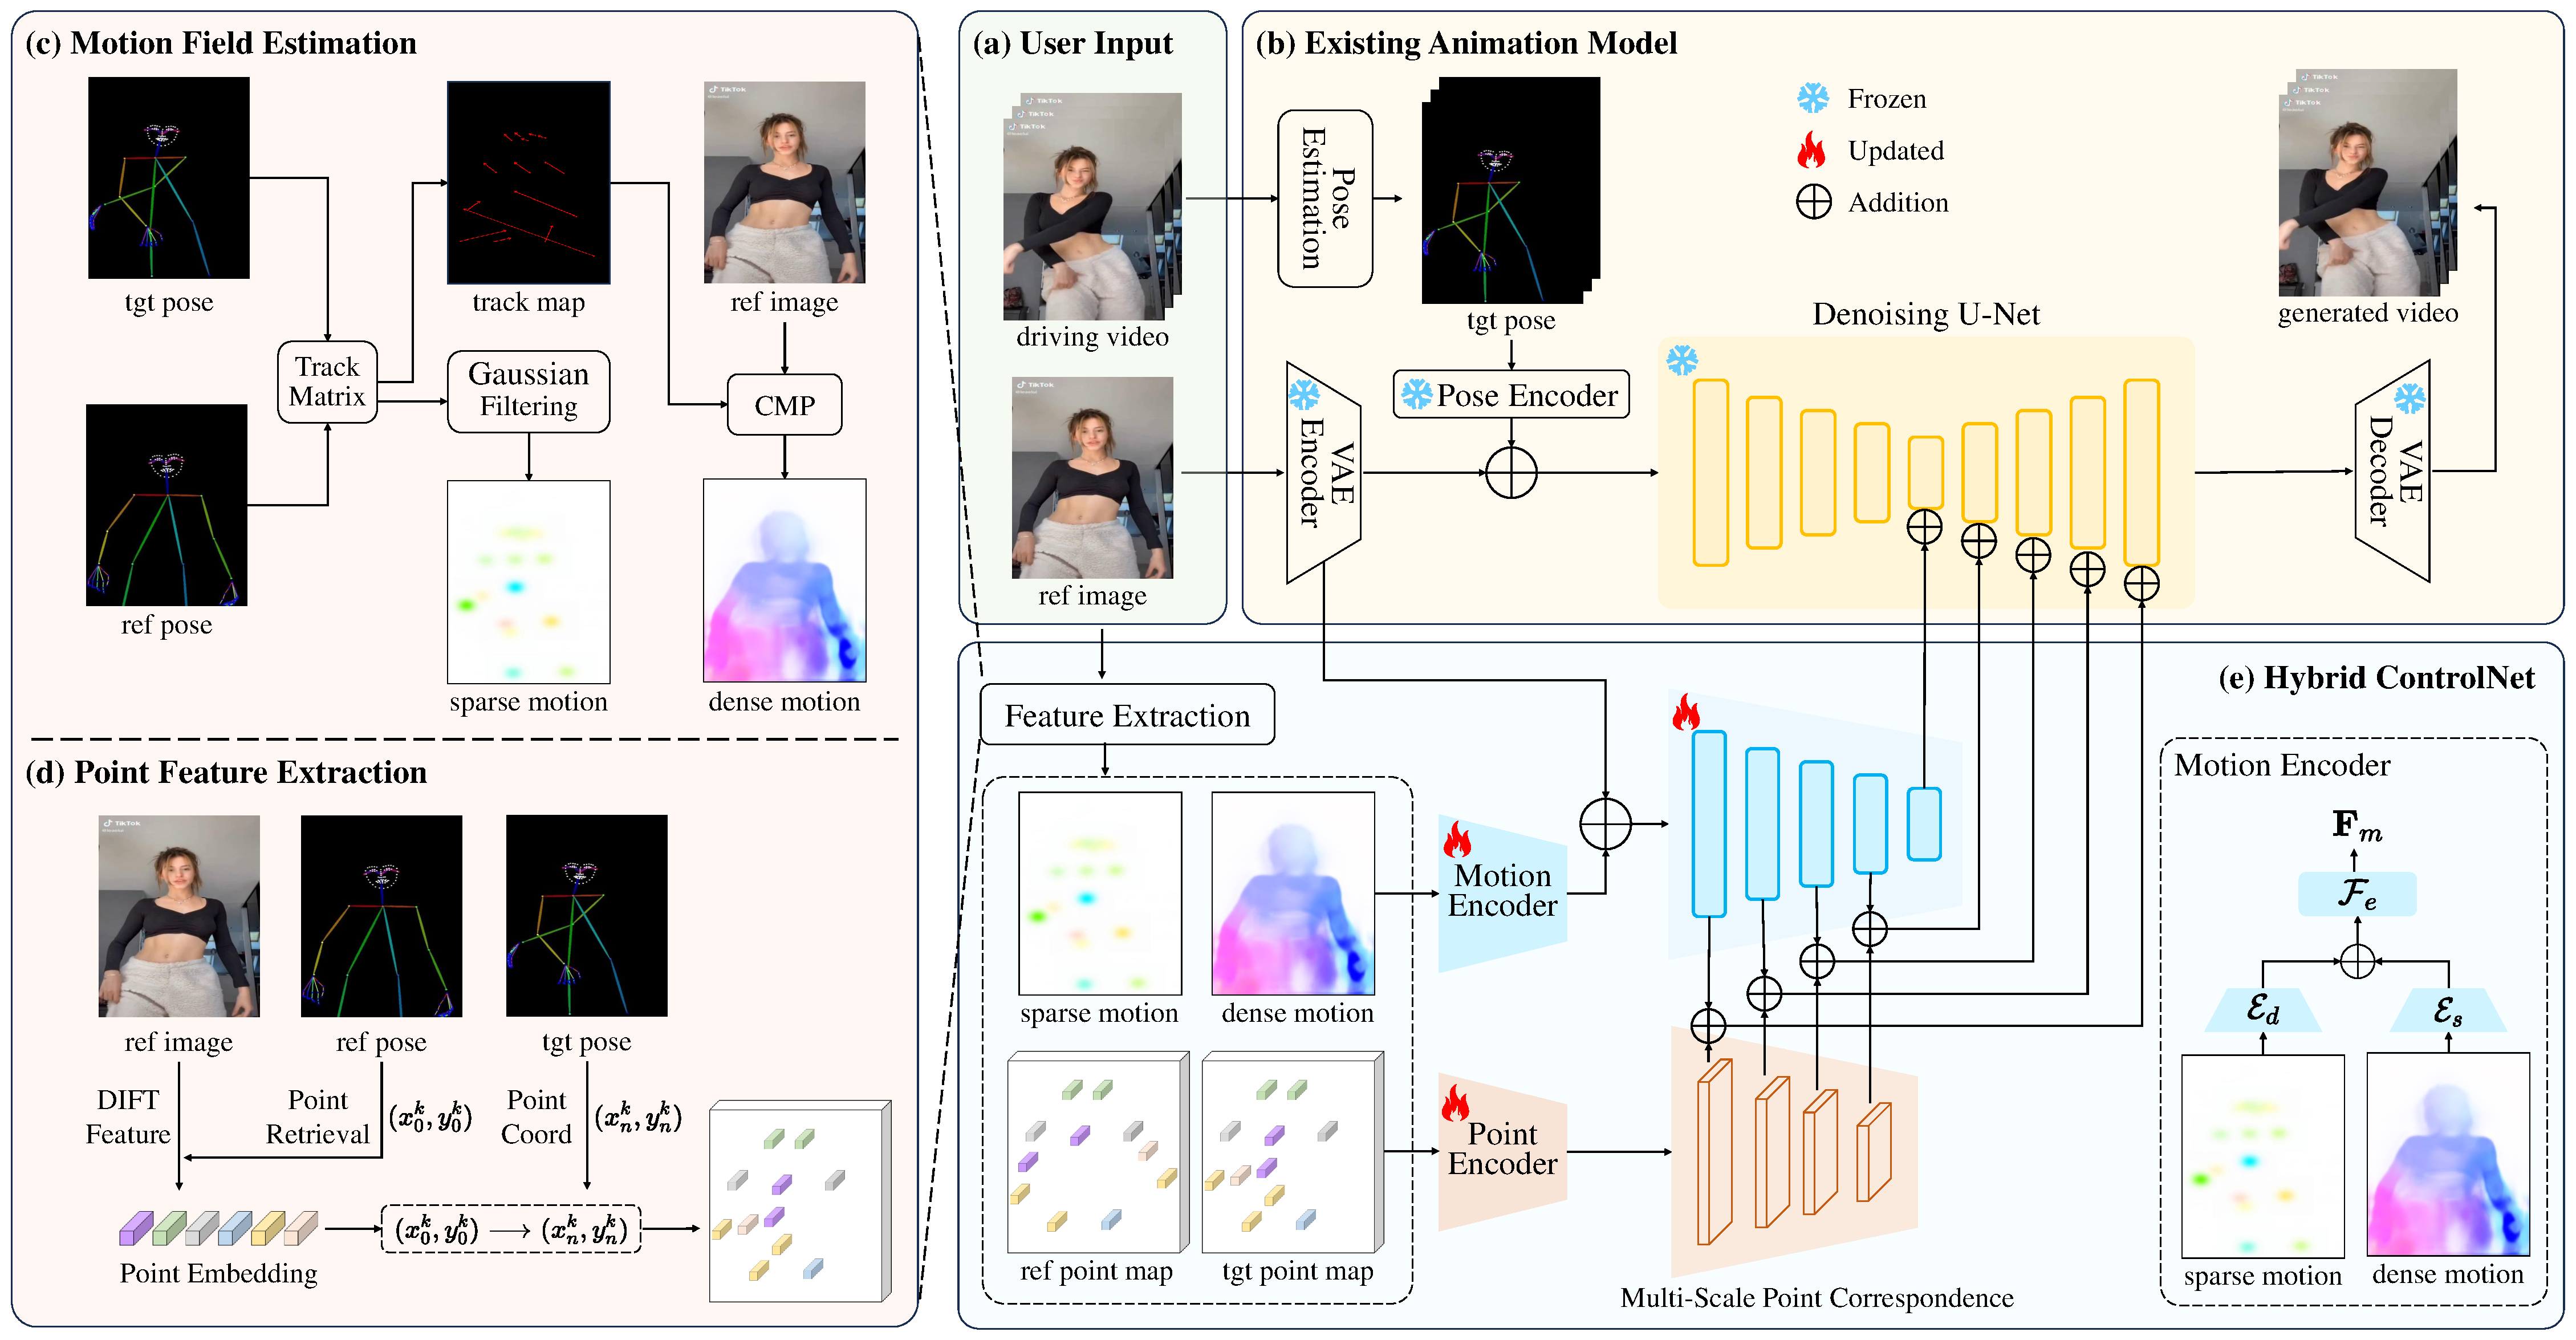
\includegraphics[width=1.0\columnwidth]{./image/pipeline.pdf}
    \vspace{-15pt}
    \caption{The overview of proposed DisPose.}
    \label{fig:pipeline}
\end{figure}
\section{DisPose}
Given a reference image $I_{\mathrm{ref}}\!\in\!\mathbb{R}^{3 \times H \times W}$ and a driving video $V\!\in\!\mathbb{R}^{N\times 3 \times H \times W}$. The core of our method is to disentangle efficient control guidance from only skeleton poses and reference images as shown in Figure~\ref{fig:pipeline}, which can be applied to existing human animation methods without additional dense inputs. We first introduce sparse and dense motion field guides in Sec.~\ref{sec: motion}. Then, we introduce reference-based keypoint correspondence in Sec.~\ref{sec: keypoint}. Finally, we introduce the pipeline of hybrid ControlNet in Sec~\ref{sec: controlnet}.
\subsection{Motion Field Guidance}
\label{sec: motion}

\textbf{Sparse Motion Field.}
We first estimate the skeleton pose by DWpose~\citep{yang2023dwpose} to obtain each frame's human key point coordinates. 
% Subsequently, the motion trajectory of all semantic points in the entire video is obtained and represented as
Subsequently, the key points of the reference image are used as starting points to track the motion displacement of all frames and represented as $P_{traj}\!=\!\{(x^k_n,y^k_n) \!\mid\! k=1\dots K, n=0\dots N\}$, where $P_{traj}$ denotes the trajectory map of the key point $k$ overall $N$ frames and $n = 0$ denotes the reference image. We calculate the track matrix $P_{s}$ as follows:
\begin{equation}
    \mathbf{P}_{s}=\{(x^k_n-x^k_{n-1}, y^k_n-y^k_{n-1}) \mid n=1\dots N\}\},
\end{equation}
% where $P_{t}$ denotes the trajectory map of the key point point $k$ over all $N$ frames, and the reference frame when $n = 0$.
where $K$ denotes the number of keypoints, $N$ denotes the number of frames, $\mathbf{P}_{s}$ denotes the trajectory map of keypoint k over all N frames, and $n = 0$ denotes the reference image.
To avoid training instability caused by overly sparse trajectory matrice, we then apply Gaussian filtering to enhance $\mathbf{P}_{s}$ to obtain the sparse motion field $\mathbf{F}_s\!\in\!\mathbb{R}^{(N-1)\times 2 \times H \times W}$ inspired by~\citep{yin2023dragnuwa, wang2024motionctrl}.

\textbf{Dense Motion Field.}
Considering that sparse control provides limited guidance and dense control is hard to obtain during inference,
% For the dense motion field, 
we transform dense guidance into the motion propagation from the reference frame to the target pose, instead of the dense signal of the target pose. Specifically, in the inference, we reconstruct the trajectory map $\mathbf{P}_{s}$ as the reference-based sparse optical flow $\mathbf{P}_{d}$ from the reference frame to each target pose as:
\begin{equation}
    \mathbf{P}_{d}=\{(x^k_n-x^k_{0}, y^k_n-y^k_{0}) \mid n=1\dots N\}\},
\end{equation}
We then predicted the reference-based dense motion filed $\mathbf{F}_d\!=\! \text{CMP}(P_{traj}, \mathbf{P}_{d}, I_{ref})\!\in\!\mathbb{R}^{(N-1)\times 2 \times H \times W}$ by condition motion propagation (CMP)~\citep{zhan2019self} based on the sparse optical flow $\mathbf{P}_{d}$ and the reference image $I_{ref}$.
CMP~\citep{zhan2019self} is a self-supervised learning-from-motion model that acquires an image and a sparse motion field and estimates the corresponding dense motion field.
Notably, the dense motion field $\mathbf{F}_d$ of each frame starts with the reference image, which avoids geometric constraints during inference.

To ensure motion estimation accuracy during training, we first extract the forward optical flow from the driving video using existing optical flow estimation models~\citep{teed2020raft, xu2023unifying}. We then use a watershed-based approach~\citep{zhan2019self} to sample the sparse optical flow $\mathbf{P}_{d}$ from the forward optical flow. See Appendix.~\ref{sec: appendix1} for details.

\textbf{Motion Encoder.} To leverage motion field as guidance, we introduce a motion encoder specifically designed for the optional flow, which includes sparse motion encoder $\mathcal{E}_s$, dense motion encoder $\mathcal{E}_d$ and feature fusion layer $\mathcal{F}_e$. $\mathcal{E}_d$ and $\mathcal{E}_s$ have the same structure and are multi-scale convolutional encoders with each stage built by \texttt{Conv-SiLU-ZeroConv}~\citep{zhang2023adding} as the basic block. The feature fusion layer $\mathcal{F}_e$ is a 2D convolution for fusing sparse motion features $\mathcal{E}_s(\mathbf{F}_s)$ and dense motion features $\mathcal{E}_d(\mathbf{F}_d)$. Finally, we compute the motion field guidance $\mathbf{F}_m$:
\begin{equation}
    \mathbf{F}_m = \mathcal{F}_e(\mathcal{E}_s(\mathbf{F}_s)+\mathcal{E}_d(\mathbf{F}_d))
\end{equation}

\subsection{Keypoint Correspondence}
\label{sec: keypoint}
\textbf{Point Feature Extraction.} 
To maintain a consistent appearance, it is crucial to correspond the content of the reference image with the motion trajectory. 
Specifically, we first extract the DIFT~\citep{tang2023emergent} features $\mathbf{D}$ of the reference image using the pre-trained image diffusion model. 

Subsequently, the keypoint embedding in the reference is obtained as $\mathbf{D}(x^k_0,y^k_0)$, where $(x^k_0,y^k_0)$ is retrieved from the reference pose.
% key point embeddings $\mathbf{D}(x^k_0,y^k_0)$ are retrieved from $\mathbf{D}$ by skeleton pose $(x^k_0, y^k_0)$.
Next, we initialize the keypoint correspondence map $\mathbf{F}_p$ with zero vectors and assign point embeddings according to the trajectory coordinates as:
\begin{equation}
\label{eq: v prob}
f^{ij}_n=\left\{\begin{array}{ll}
\mathbf{D}(x^k_0,y^k_0), & \mathrm{if} \quad i=x^k_n, j=y^k_n,  \\
0, & \mathrm{otherwise}.
\end{array}\right.
\end{equation}

Finally, we obtain the keypoint correspondence map $\mathbf{F}_p=\{f_n\!\mid\!n=1\dots N\} \!\in\!\mathbb{R}^{N\times D_p \times H \times W}$ for all frames, where $D_p$ is the feature dimension of the point embedding.

\textbf{Point Encoder.} 
To utilize the content correspondence of key points as guidance, we generate multi-scale correspondences of sparse point feature maps and make them compatible with the U-Net encoder of the {Hybrid ControlNet (Sec.4.3)}. 
% as detailed in F. 1.
We introduce the multi-scale point encoder $\mathcal{E}_p$ to maintain the key point content $\mathbf{F}_p$ from the reference image. The point encoder $\mathcal{E}_p$ consists of a series of learnable MLPs.
{
To seamlessly integrate into existing models, we extract intermediate features of the encoder of the hybrid Controlnet.
The multi-scale intermediate features of the Controlnet encoder are denoted as $\mathbf{E}^l_{enc}$, where $l$ denotes each U-Net block $l\!\in\![1, L]$.}
To match the spatial size of $\mathbf{E}^l_{enc}$, we apply downsampling to the feature map between the encoder layers. We compute the multi-scale keypoint correspondence as follows:
\begin{equation}
    \mathbf{F}_c^l = \mathcal{E}_p^l(\phi(\mathbf{F}_p, H^l, W^l)),
\end{equation}
where $(H^l, W^l)$ are denote the spatial dimension of the $l$-th U-Net block and $\phi$ means downsampling operation. Therefore, $\mathbf{F}_c^l$ shares the same size as $\mathbf{E}^l_{enc}$.
Finally, $\mathbf{F}_c$ are added elementwisely to the intermediate feature $\mathbf{E}^l_{enc}$ of the U-Net encoder as guidance: $\mathbf{E}^l_{enc}\!=\!\mathbf{E}^l_{enc}+\mathbf{F}_c^l$.


\subsection{Plug-and-play Hybrid ControlNet}
\label{sec: controlnet}
After obtaining motion field guidance and keypoint correspondence, we aim to integrate these control guidance seamlessly into the U-Net architecture of existing animation models.
Inspired by ControlNet~\citep{zhang2023adding}, We design a hybrid ControlNet $\mathcal{F}$ to provide additional control signals for the existing animation model as shown in Figure~\ref{fig:pipeline}(e).
% Specifically, we consider freeze denoising U-Net and pose encoder. 
Specifically, given an animation diffusion model based on the U-Net architecture, we freeze all its modules while allowing the motion encoder, point encoder and hybrid ControlNet to be updated during training. 
Subsequently, $\mathbf{F}_m$ is added to the noise latent before being input into the hybrid ControlNet. Considering the high sparsity of the point feature $\mathbf{F}_c$, we correspondingly add $\mathbf{F}_c$ to the input of the convolutional layer. Notably, the U-Net encoder intermediate feature $\mathbf{E}_{enc}$ in Sec.~\ref{sec: keypoint} is from hybrid ControlNet rather than denoising U-Net. Finally, 
the control condition is computed as:
\begin{equation}
    \boldsymbol{r}=\mathcal{F}(\boldsymbol{z}_{{t}} \mid \mathbf{F}_m, \mathbf{F}_c, {t})
\end{equation}
where $\boldsymbol{r}$ is a set of condition residuals added to the residuals for the middle and upsampling blocks in the denoising U-Net.
\section{Experimental Setup}

We evaluate our proposed framework on three multi-hop QA datasets in the open-domain setting: \textbf{MuSiQue} (answerable subset) \cite{Trivedi2022}, \textbf{HotpotQA} \cite{Yang2018}, and \textbf{2WikiMultiHopQA} (2Wiki) \cite{Ho2020}.
For MuSiQue and 2Wiki, we use the data splits provided in IRCoT \cite{Trivedi2023}, while for HotpotQA we follow the same data setting as in HippoRAG \cite{Gutierrez2024}. Dataset-specific statistics can be found in Appendix \ref{appendix:dataset_stats}.

We measure both retrieval and QA performance, with our primary contributions focused on the retrieval component. For retrieval evaluation, we use Recall@$k$ (R@$k$) metrics for $k \in \left \{5, 10, 15\right \}$, showing the percentage of questions where the correct entries are found within the top-$k$ retrieved passages. We include an analysis about the selected recall ranks in Appendix \ref{appendix:reasoning_behind_retrieval_metrics}. Following standard practices, QA performance is evaluated with Exact Match (EM) and F1 scores \cite{Trivedi2023}.


\begin{table*}[t]
\small
\centering
\small
\begin{tabular}{@{}l@{\hspace{2pt}}lccccccccc@{}}
\toprule
& \multirow{2.5}{*}{\textbf{Retriever}} & \multicolumn{3}{c}{\textbf{MuSiQue}} & \multicolumn{3}{c}{\textbf{2Wiki}} & \multicolumn{3}{c}{\textbf{HotpotQA}}\\ 
\cmidrule{3-11}
& & R@5 & R@10 & R@15 & R@5 & R@10 & R@15 & R@5 & R@10 & R@15 \\ \midrule
\multirow{11}{*}{\parbox{2cm}{\textbf{Single-step\\Retrieval}}}
& ColBERTv2 & $39.4$ & $44.8$ & $47.7$ & $59.1$ & $64.3$ & $66.2$ & $79.3$ & $87.1$ & $90.1$ \\
& HippoRAG & $41.0$ & $47.0$ & $51.4$ & $\mathbf{75.1}$ & $\mathbf{83.2}$ & $\mathbf{86.4}$ & $79.8$ & $89.0$ & $92.4$ \\ 
& BM25 & $33.8$ & $38.5$ & $41.3$ & $59.5$ & $62.7$ & $64.1$ & $74.2$ & $83.6$ & $86.3$ \\ 
& \hspace{2mm} + NaiveGE & $37.5$ & $45.5$ & $48.4$ & $65.0$ & $70.7$ & $71.8$ & $79.1$ & $89.1$ & $91.9$ \\ 
& \hspace{2mm} + SyncGE & $\underline{44.7}$ & $\underline{52.6}$ & $\underline{57.4}$ & $70.5$ & $76.1$ & $79.3$ & $\underline{87.4}$ & $\underline{93.0}$ & $\underline{94.0}$ \\ 
& SBERT & $31.1$ & $37.9$ & $41.6$ & $41.2$ & $48.1$ & $51.5$ & $72.1$ & $79.3$ & $84.0$ \\
& {\hspace{2mm} + NaiveGE} & $32.2$ & $41.4$ & $45.4$ & $45.1$ & $54.0$ & $57.3$ & $76.1$ & $84.7$ & $88.8$ \\
& \hspace{2mm} + SyncGE & $41.6$ & $51.3$ & $54.2$ & $54.8$ & $64.9$ & $70.7$ & $84.1$ & $89.6$ & $92.8$ \\ 
& Hybrid & $39.9$ & $46.3$ & $49.1$ & $60.0$ & $65.8$ & $66.6$ & $77.8$ & $85.8$ & $89.7$ \\
& \hspace{2mm} + NaiveGE & $41.8$ & $49.4$ & $53.0$ & $63.0$ & $70.8$ & $72.6$ & $80.6$ & $89.4$ & $92.7$ \\
& {\hspace{2mm} + SyncGE} & $\mathbf{48.7}$ & $\mathbf{57.7}$ & $\mathbf{61.2}$ & $\underline{72.6}$ & $\underline{80.9}$ & $\underline{82.4}$ & $\mathbf{87.4}$ & $\mathbf{93.3}$ & $\mathbf{95.2}$ \\ 
\midrule
\multirow{4}{*}{\parbox{2cm}{\textbf{Multi-step}\\ \textbf{Retrieval}}}
& IRCoT (BM25) & $46.1$ & $\underline{54.9}$ & $57.9$ & $67.9$ & $75.5$ & $76.1$ & $87.0$ & $92.6$ & $92.9$ \\
& IRCoT (ColBERTv2) & $47.9$ & $54.3$ & $56.4$ & $60.3$ & $86.6$ & $69.7$ & $86.9$ & $92.5$ & $92.8$ \\
& HippoRAG w$/$ IRCoT
& $\underline{48.8}$ & $54.5$ & $\underline{58.9}$ & $\underline{82.9}$ & $\underline{90.6}$ & $\underline{93.0}$ & $\underline{90.1}$ & $\underline{94.7}$ & $\underline{95.9}$ \\
& \gear & $\mathbf{58.4}$ & $\mathbf{67.6}$ & $\mathbf{71.5}$ & $\mathbf{89.1}$ & $\mathbf{95.3}$ & $\mathbf{95.9}$ & $\mathbf{93.4}$ & $\mathbf{96.8}$ & $\mathbf{97.3}$ \\ \bottomrule
\end{tabular}
 \caption{Retrieval performance for single- and multi-step retrievers on MuSiQue, 2Wiki, and HotpotQA. Results are reported using Recall@$k$ (R@$k$) metrics for $k \in \left \{5, 10, 15\right \}$, showing the percentage of questions where the correct entries are found within the top-$k$ retrieved passages.}
 \label{tab:recall_main_table}
\end{table*}

\subsection{Baselines}
We evaluate \gear against strong, multi-step baselines, including IRCoT \cite{Trivedi2023} and a combination of HippoRAG w$/$ IRCoT \cite{Gutierrez2024} which, similar to our framework, includes a graph-retrieval component and a multi-step agent. To showcase the benefits of our graph retriever (i.e. SyncGE), we evaluate it against several stand-alone, single-step retrievers: \begin{inparaenum}[(i)]\item BM25, \item Sentence-BERT (SBERT), \item a hybrid approach that combines BM25 and SBERT results through RRF and \item HippoRAG\end{inparaenum}. Throughout the experiments, we refer to the single-step setup when an approach does not support several iterations and is not equipped with an LLM agent.





\subsection{Implementation Details}
To maintain consistency and validity in comparisons with the baselines on the splits used in this study, we conducted all experiments locally using their corresponding codebases.

In addition to our proposed single-step retriever, SyncGE, we evaluate a more \textit{naive} implementation of GE (i.e. NaiveGE) in order to explore the generality of the method when in resource-constrained setting, where no LLM is involved. In NaiveGE, we use all triples that are associated with $\mathbf{C}_\mathbf{q}'$ (see Section~\ref{sec:graph_retrieval}) for diverse triple beam search.


For all models using an LLM, we employ GPT-4o mini (\texttt{gpt-4o-mini-2024-07-18}) as the backbone model with a temperature of 0, both for offline triple extraction (i.e. how the $\mathbf{T}$ index in Section~\ref{sec:preliminaries} is formed) and online retrieval operations. Our triple extraction prompt (in Appendix \ref{sec:offline_prompts}) is adapted\footnote{Our approach uses a modified version of HippoRAG's triple extraction prompt that combines entity and triple extraction into a single step, while incorporating an additional demonstration and updated in-context examples.} from the ones used by \citeauthor{Gutierrez2024}. To ensure a fair comparison against \citeauthor{Gutierrez2024}, the closest work to ours, we run experiments with HippoRAG using our prompting setup\footnote{For transparency, we also compare against HippoRAG's original triple extraction prompt in Appendix \ref{appendix_sec:hipporag_results_original_prompt}, where we observe only minor differences across the two configurations.} for triple extraction. For evaluating QA performance, we use the prompts provided in Appendix~\ref{subsec:online_qa_prompts}. Further implementation details are provided in Appendix~\ref{appendix:detailed_implementation_details}.

\section{Empirical Evaluation}
We trained a series of models of various sizes. For all subsequent evaluations, we will use the largest model (referred to as CogVideoX).
In this section, we present the experimental validation of CogVideoX through two primary methods: automated metric evaluation and human assessment, providing a thorough analysis of the performance and quality of the generated videos. 
We trained a series of models with different parameter sizes. The following evaluation defaults to using our largest model.

\subsection{Results of Automated Metric Evaluation} 

\paragraph{Baselines.} We chose several top-performing text-to-video models as our baselines for comparison, including T2V-Turbo~\citep{li2024t2v}, AnimateDiff~\citep{guo2023animatediff}, VideoCrafter2~\citep{chen2024videocrafter2}, OpenSora~\citep{opensora}, Show-1~\citep{zhang2023show}, Gen-2~\citep{gen2}, Pika~\citep{pika} and LaVie-2~\citep{wang2023lavie}.


% \begin{figure}[h]
% \begin{center}
% \includegraphics[width=0.9\linewidth]{images/bench_eval.png}
% \end{center}
% \caption{The radar chart comparing the performance of different models.}
% \label{fig:radar}
% \end{figure}

\hide{
%\begin{wrapfigure}{r}{0.5\textwidth}
\begin{figure}
\centering
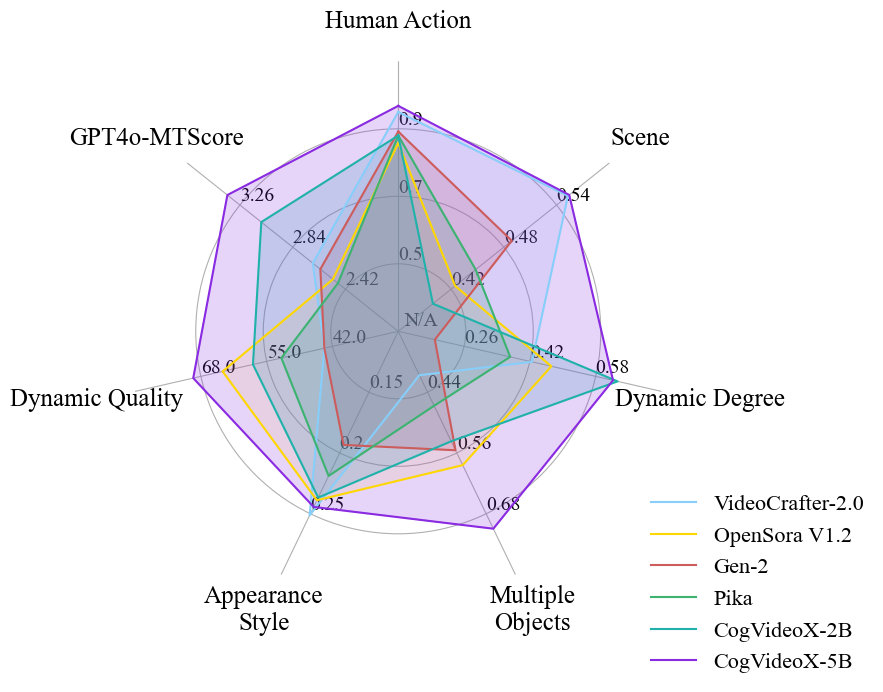
\includegraphics[width=0.7\linewidth]{images/bench_eval9.png}
\caption{The radar chart comparing the performance of different models. CogVideoX represents the largest one. It is clear that CogVideoX outperforms its competitors in the vast majority of metrics, and it is very close to the leading models in the remaining indicator.
}
\label{fig:radar}
% \vspace{-10mm}
%\end{wrapfigure}

\end{figure}

}%end ofhide
\paragraph{Evaluation Metrics.} To evaluate the text-to-video generation, we employed several metrics from VBench~\citep{huang2023vbench}: \emph{Human Action}, \emph{Scene}, \emph{Dynamic Degree}, \emph{Multiple Objects}, and \emph{Appearance Style}. VBench is a suite of tools designed to automatically assess the quality of generated videos. We have selected certain metrics from VBench, excluding others that do not align with our evaluation needs. For example, the color metric, intended to measure the presence of objects corresponding to specific colors across frames in the generated video, assesses the model's quality by calculating the probability. However, this metric may mislead video generation models that exhibit greater variation, thus we chose not to include it in our evaluation. For longer-generated videos, some models might produce videos with minimal changes between frames to obtain higher scores, but these videos lack rich content. Therefore, a metric for evaluating the dynamism of the video becomes more important. To address this, we employed two video evaluation tools, We also employed the \emph{Dynamic Quality} from Devil~\citep{liao2024evaluationtexttovideogenerationmodels} and \emph{GPT4o-MTScore} from ChronoMagic~\citep{yuan2024chronomagic}, which focus more on the dynamic characteristics of videos. \emph{Dynamic Quality} is defined by the integration of various quality metrics with dynamic scores. This approach mitigates biases arising from negative correlations between video dynamics and video quality, leading to a more thorough assessment of video quality. ChronoMagic, for instance, introduces the \emph{GPT4o-MTScore}, a metric designed to measure the metamorphic amplitude of time-lapse videos, such as those depicting physical, biological, and meteorological changes. This metric is obtained by extracting frames from the generated videos at regular intervals and using GPT-4o~\citep{gpt4o} to score the degree of change, providing a fine-grained assessment of video dynamism. This method ensures a more accurate evaluation of the content's variability over time, countering the potential bias of static frame sequences in scoring.



\paragraph{Results.} Table~\ref{table:results} provides a detailed comparison of the performance of our CogVideoX model with other models. Our model achieved the best performance in 5 out of the 7 metrics and showed competitive results in the remaining 2 metrics. These results demonstrate that our model not only excels in video generation quality but also outperforms previous models in handling various complex dynamic scenes. Additionally, Figure~\ref{fig:radar} presents a radar chart comparing the performance of different models.


\begin{figure}[ht]
\begin{center}
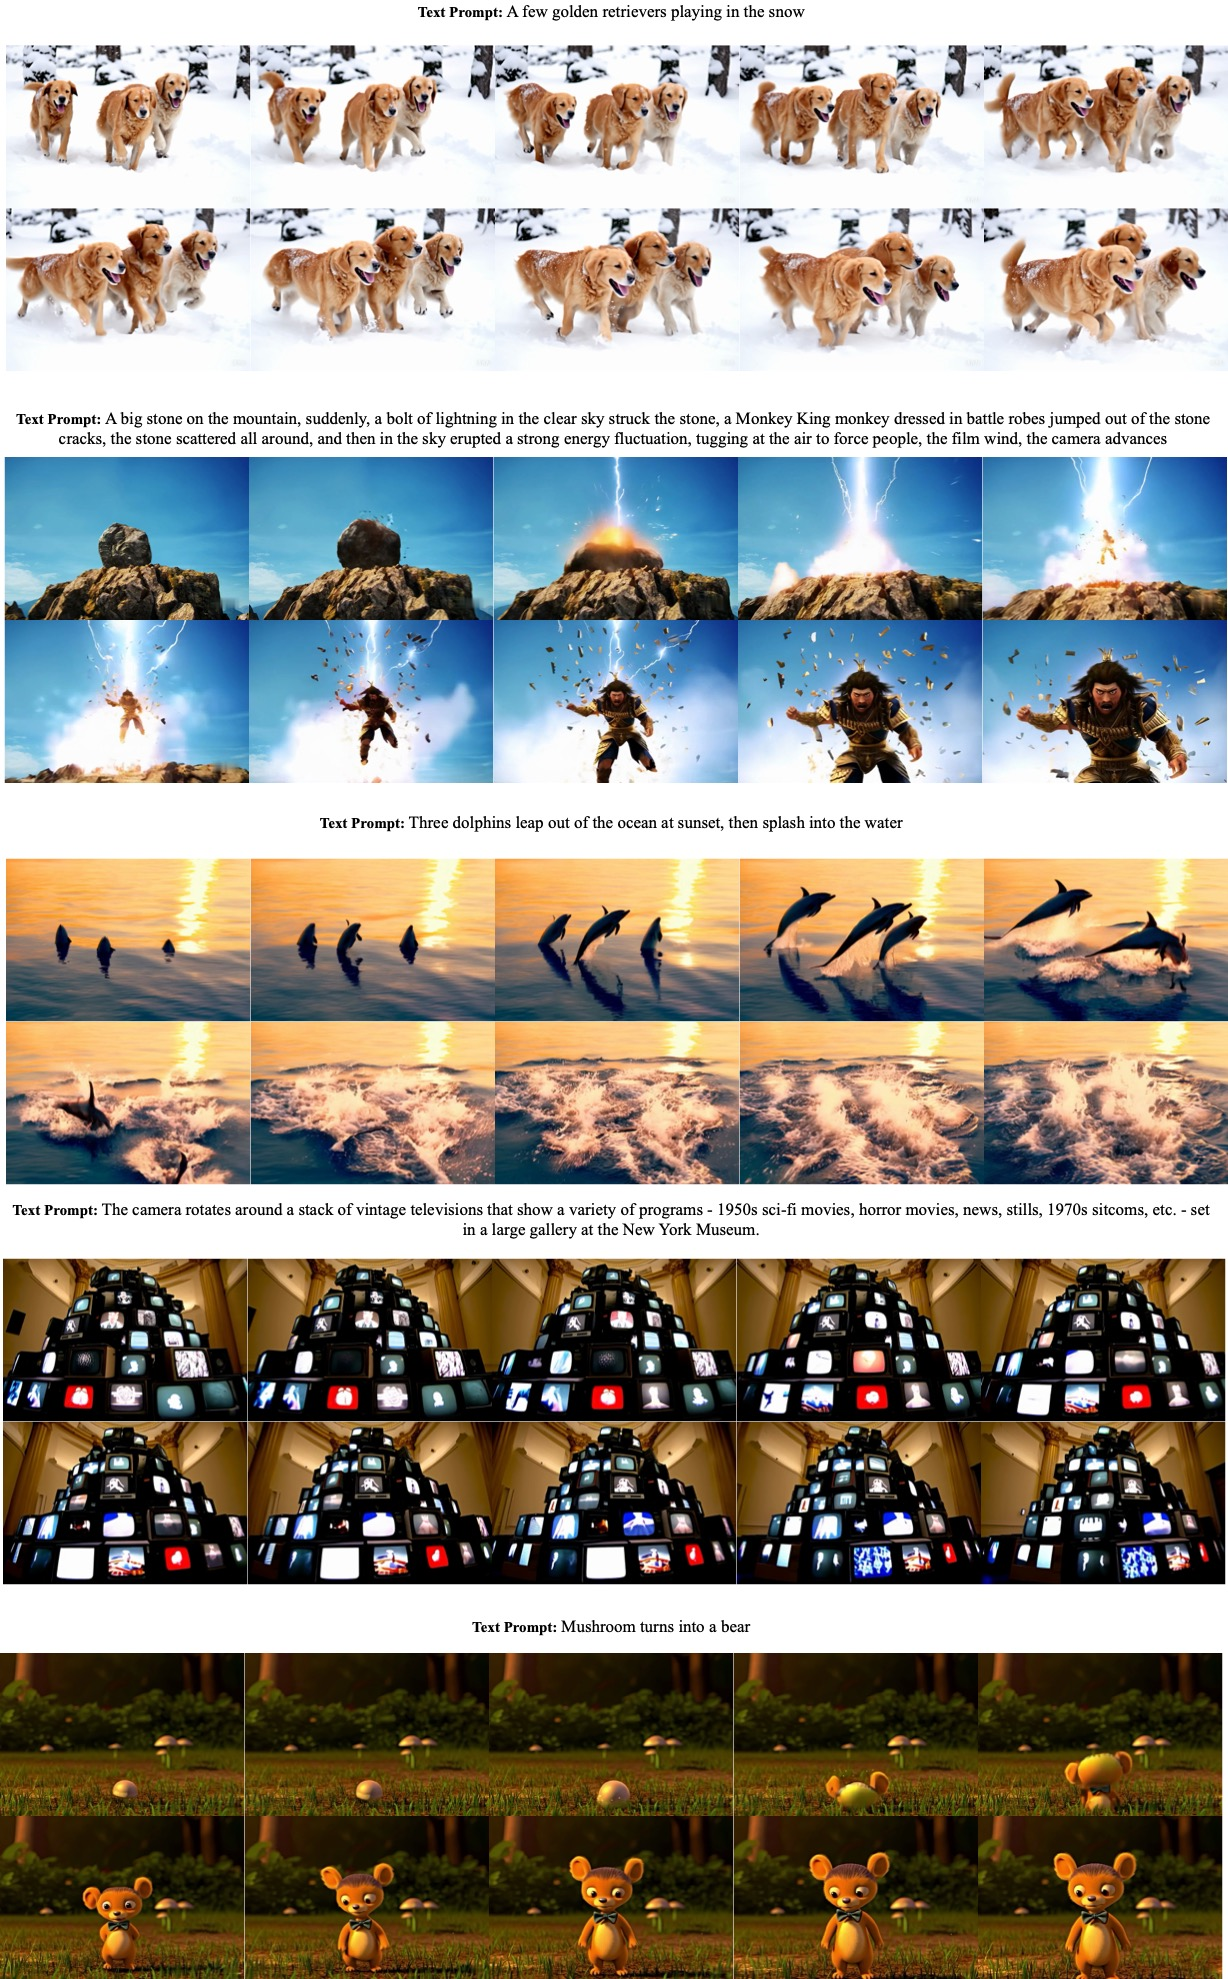
\includegraphics[width=\linewidth]{images/t2v/goodcase1.jpg}
\end{center}
\caption{Text to video showcases. The displayed prompt will be upsampled before being fed into the model. The generated videos contain large motion and can produce various video styles.}
\label{fig:t2vgood1}
\end{figure}

\begin{figure}[ht]
\begin{center}
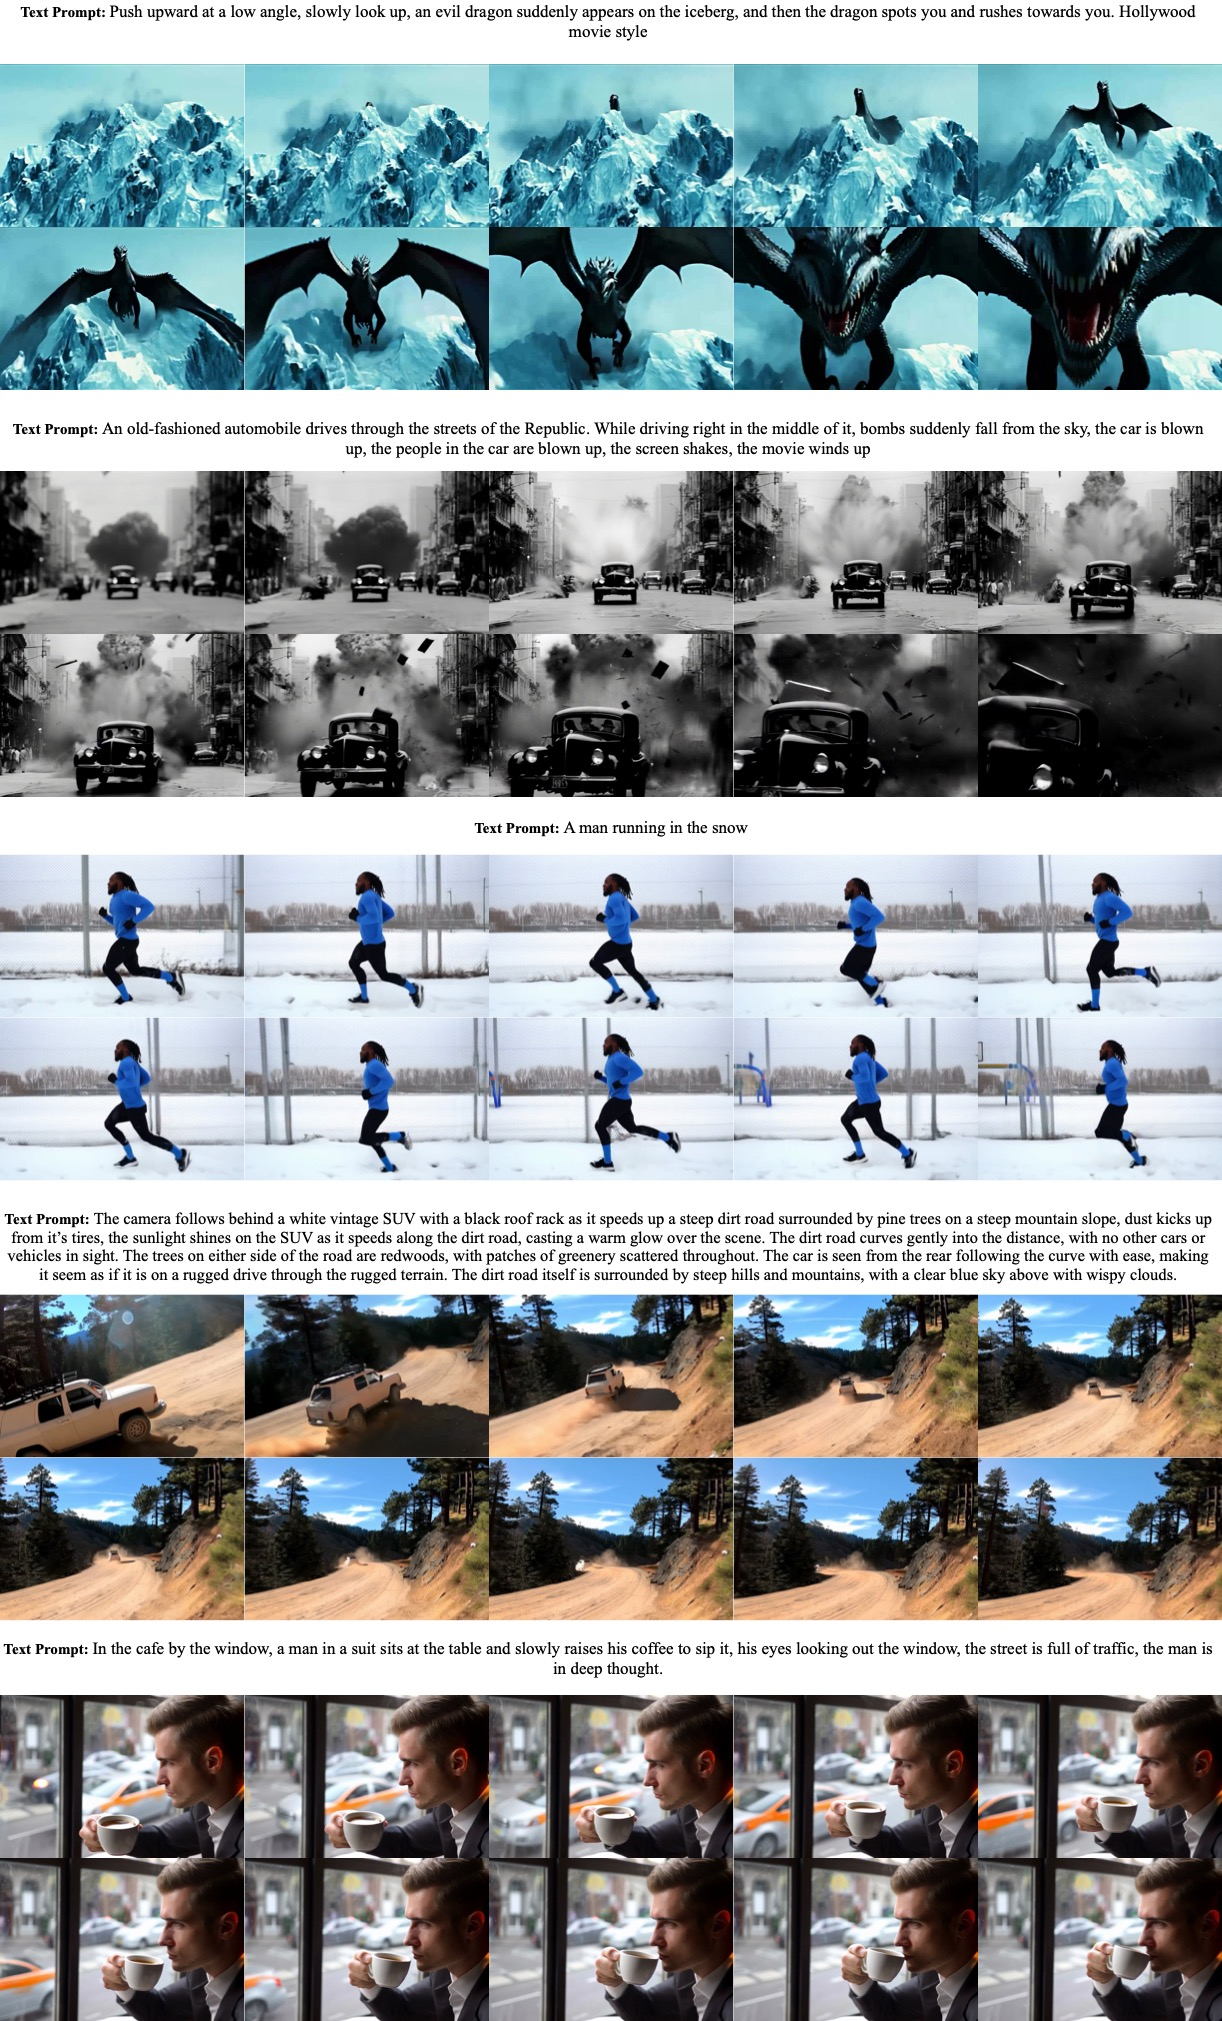
\includegraphics[width=0.98\linewidth]{images/t2v/goodcase2.jpg}
\end{center}
\caption{Text to video showcases.}
\label{fig:t2vgood2}
\end{figure}


% Please add the following required packages to your document preamble:
% \usepackage[table,xcdraw]{xcolor}
% Beamer presentation requires \usepackage{colortbl} instead of \usepackage[table,xcdraw]{xcolor}
% \usepackage[normalem]{ulem}
% \useunder{\uline}{\ul}{}




% \begin{table}[]

% \centering
% \setlength\tabcolsep{3pt}

% \label{sample-table}
% \small
% \vspace{-10pt}
% \caption{\textbf{Automatic Evaluation Results per Dimension.}The table presents a comparative analysis of various video models across different dimensions. It is evident from the table that, in terms of both human motion and background effects as well as the accuracy and distinctiveness of objects, CogVideoX has achieved the current SOTA level. Furthermore, CogVideoX has garnered a commendable score in the expression of dynamic qualities, a capability that serves as a more precise indicator of the intrinsic properties of video media, distinct from the static nature of photographic images.}

% \vspace{6pt}

% \begin{tabular}{cccccccc}
% \toprule
% \multirow{2}{*}{\textbf{Models} }  & \textbf{human}  & \textbf{object} &\multirow{2}{*}{\textbf{scene}}&\textbf{dynamic} &\textbf{multiple} &\textbf{spatial} &\textbf{appearance} \\
%     & \textbf{action}& \textbf{class}& & \textbf{degree} &\textbf{objects}& \textbf{relationship}&\textbf{style}  
% \\
% \midrule
% CogVideoX & 96.80\% &93.70\% & 55.44\% & 62.22\% & 70.95\% & 61.29\% & 24.44\% \\
% {LaVie-2} & 96.40\% & 97.52\%  & 49.59\% & 31.11\% & 64.88\%  & 38.68\% & 25.09\%  \\
% {T2V-Turbo}  & 95.20\%  & 93.96\%& 55.58\% & 49.17\% & 54.65\%    & 38.67\%  & 24.42\%   \\
% {Gen-2}  & 89.20\%& 90.92\%  & 48.91\%  & 18.89\% & 55.47\%    & 66.91\%   & 19.34\%  \\
% {VideoCrafter-2.0\citep{chen2024videocrafter2}} & 95.00\% & 92.55\% & 55.29\%               & 42.50\% & 40.66\% & 35.86\% & 25.13\%  \\
% {Pika Beta} & 88.00\% & 87.45\%  & 44.80\% & 37.22\% & 46.69\% & 65.65\% & 21.89\%   \\
% AnimateDiff-V2 & 92.60\% & 90.90\%  & 50.19\% & 40.83\%        & 36.88\% & 34.60\%  & 22.42\%\\
% {OpenSora V1.2}   & 85.80\% & 83.37\%& 42.47\%   & 47.22\%    & 58.41\% & 67.51\%  & 23.89\%  \\
% {Show-1} & 95.60\%  & 93.07\%  & 47.03\% & 44.44\% & 45.47\% & 53.50\%  & 23.06\%  \\
% {HiGen}  & 86.20\%  & 86.06\%  & 44.88\% & 99.17\% & 22.39\%  & 22.43\% & 24.54\% \\  
% \bottomrule
% \end{tabular}
% \end{table}



% \iffalse



% \begin{table}[ht!]
% \centering
% \caption{Evaluation results.}
% \setlength\tabcolsep{3pt}
% \label{sample-table}
% \begin{center}
% \small
% \resizebox{0.9\linewidth}{!}{
% \begin{tabular}{ccccccccc}

% \multirow{2}{*}{\textbf{Models} }  & \textbf{subject}  & \textbf{background} &\textbf{temporal} &\textbf{motion} &\textbf{dynamic} &\textbf{aesthetic} &\textbf{imaging} &\textbf{object} \\
%     & \textbf{consistency}& \textbf{consistency}& \textbf{flickering}& \textbf{smoothness} &\textbf{degree}& \textbf{quality}&\textbf{quality} & \textbf{class}
% \\ \hline 
%         CogVideoX & 94.66\% & 95.92\% & 97.47\% & 98.10\% & 62.22\% & 55.14\% & 63.62\% & 93.70\%  \\
%         LaVie-2 & 97.90\% & 98.45\% & 98.76\% & 98.42\% & 31.11\% & 67.62\% & 70.39\% & 97.52\%  \\ 
%         T2V-Turbo (VC2) & 96.28\% & 97.02\% & 97.48\% & 97.34\% & 49.17\% & 63.04\% & 72.49\% & 93.96\%  \\ 
%         Gen-2 (2023-06) & 97.61\% & 97.61\% & 99.56\% & 99.58\% & 18.89\% & 66.96\% & 67.42\% & 90.92\%  \\ 
%         VideoCrafter-2.0\citep{chen2024videocrafter2} & 96.85\% & 98.22\% & 98.41\% & 97.73\% & 42.50\% & 63.13\% & 67.22\% & 92.55\%  \\ 
%         Pika Beta (2023-06) & 96.76\% & 98.95\% & 99.77\% & 99.51\% & 37.22\% & 63.15\% & 62.33\% & 87.45\%  \\ 
%         AnimateDiff-V2 & 95.30\% & 97.68\% & 98.75\% & 97.76\% & 40.83\% & 67.16\% & 70.10\% & 90.90\%  \\ 
%         OpenSora V1.2 & 94.45\% & 97.90\% & 99.47\% & 98.20\% & 47.22\% & 56.18\% & 60.94\% & 83.37\%  \\ 
%         Show-1 & 95.53\% & 98.02\% & 99.12\% & 98.24\% & 44.44\% & 57.35\% & 58.66\% & 93.07\%  \\ 
%         HiGen & 90.07\% & 93.99\% & 93.24\% & 96.69\% & 99.17\% & 57.30\% & 63.92\% & 86.06\% \\ 
% \hline \\

% \multirow{2}{*}{\textbf{Models} }  & \textbf{multiple}  & \textbf{human} &\multirow{2}{*}{\textbf{color}} &\textbf{spatial} &\multirow{2}{*}{\textbf{scene}} &\textbf{appearance} &\textbf{temporal} &\textbf{overall} \\
%     & \textbf{objects}& \textbf{action}& & \textbf{relation} & & \textbf{style}&\textbf{style} & \textbf{consistency}
% \\ \hline 
%         CogVideoX & 70.95\% & 96.80\% & 79.75\% & 61.29\% & 55.44\% & 24.44\% & 23.69\% & 26.73\%  \\ 
%         LaVie-2 & 64.88\% & 96.40\% & 91.65\% & 38.68\% & 49.59\% & 25.09\% & 25.24\% & 27.39\%  \\ 
%         T2V-Turbo (VC2) & 54.65\% & 95.20\% & 89.90\% & 38.67\% & 55.58\% & 24.42\% & 25.51\% & 28.16\%  \\
%         Gen-2 (2023-06) & 55.47\% & 89.20\% & 89.49\% & 66.91\% & 48.91\% & 19.34\% & 24.12\% & 26.17\%  \\ 
%         VideoCrafter-2.0 & 40.66\% & 95.00\% & 92.92\% & 35.86\% & 55.29\% & 25.13\% & 25.84\% & 28.23\%  \\
%         Pika Beta (2023-06) & 46.69\% & 88.00\% & 85.31\% & 65.65\% & 44.80\% & 21.89\% & 24.44\% & 25.47\%  \\ 
%         AnimateDiff-V2 & 36.88\% & 92.60\% & 87.47\% & 34.60\% & 50.19\% & 22.42\% & 26.03\% & 27.04\%  \\ 
%         OpenSora V1.2 & 58.41\% & 85.80\% & 87.49\% & 67.51\% & 42.47\% & 23.89\% & 24.55\% & 27.07\%  \\ 
%         Show-1 & 45.47\% & 95.60\% & 86.35\% & 53.50\% & 47.03\% & 23.06\% & 25.28\% & 27.46\%  \\ 
%         HiGen & 22.39\% & 86.20\% & 86.22\% & 22.43\% & 44.88\% & 24.54\% & 25.14\% & 27.14\% \\ \hline

% \hline \\
% \end{tabular}

% }
% \end{center}
% \end{table}

% \fi






% \begin{table}[!ht]
% \centering

% \label{sample-table}
% \small
% \vspace{-10pt}
% \caption{\textbf{Automatic Evaluation Results per Dimension.}}

% \vspace{6pt}

% \resizebox{0.8\linewidth}{!}{
%     \begin{tabular}{cccc}
%         \textbf{Models} & \textbf{\Centerstack{Dynamics Range}} & \textbf{\Centerstack{Dynamics Controllability}} & \textbf{\Centerstack{Dynamics-based Quality}} \\ \hline
%         CogVideoX       & 55.7 & 71.8 & \textbf{69.5} \\ 
%         Gen-2           & 30.8 & \textbf{82.5} & 43.6 \\ 
%         Pika            & 43.2 & 72.0 & 52.1 \\ 
%         VideoCrafter2   & 34.1 & 57.0 & 43.6 \\ 
%         OpenSora        & \textbf{61.2} & 62.4 & 63.7 \\ 
%         Show-1          & 45.1 & 73.9 & 57.7 \\ 
%     \end{tabular}
% }
% \end{table}


% \begin{figure}[h]
% \begin{center}
% \includegraphics[width=0.9\linewidth]{images/bench_eval.png}
% \end{center}
% \caption{The radar chart comparing the performance of different models.}
% \label{fig:radar}
% \end{figure}

\hide{
%\begin{wrapfigure}{r}{0.5\textwidth}
\begin{figure}
\centering
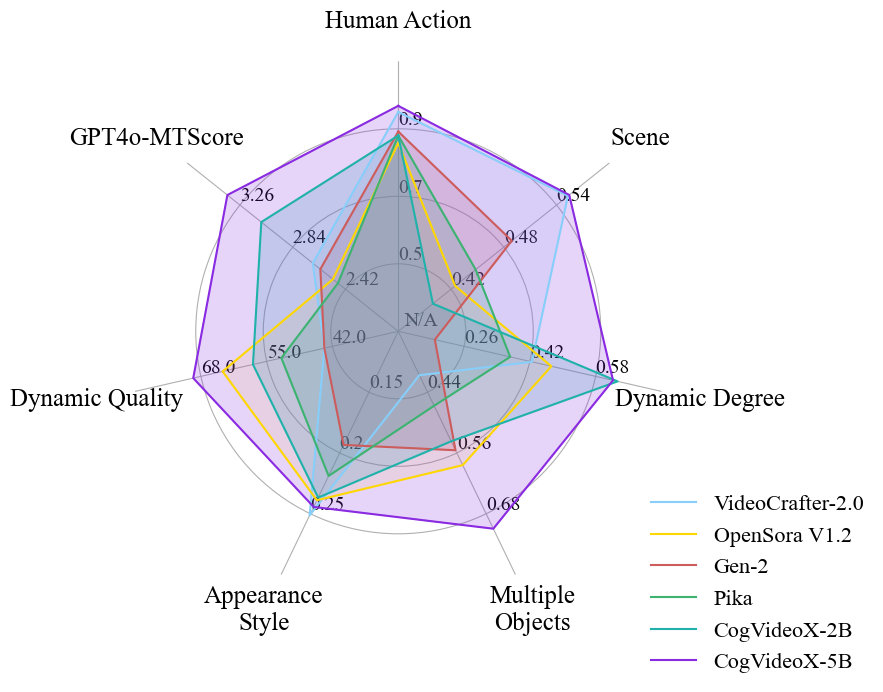
\includegraphics[width=0.7\linewidth]{images/bench_eval9.png}
\caption{The radar chart comparing the performance of different models. CogVideoX represents the largest one. It is clear that CogVideoX outperforms its competitors in the vast majority of metrics, and it is very close to the leading models in the remaining indicator.
}
\label{fig:radar}
% \vspace{-10mm}
%\end{wrapfigure}

\end{figure}

}%end ofhide


\subsection{Human Evaluation}
In addition to automated scoring mechanisms, a comparative analysis between the Kling~\citep{kling} and CogVideoX was conducted using a manual scoring system. One hundred meticulously crafted prompts were used, characterized by their broad distribution, clear articulation, and well-defined conceptual scope. We randomize videos for blind evalution. A panel of evaluators assigned scores for each detail on a scale from zero to one, with the overall total score rated on a scale from zero to five, where higher scores reflect better video quality. Reasons for any score deductions were also carefully documented. The results shown in Table~\ref{table:human_eva} indicate that our model outperforms Kling in all aspects. More details are shown in \ref{sec:human_evalution}.

\begin{table}[!ht]
\centering
\label{sample-table}
\small
\vspace{-5pt}
\caption{Human evaluation between CogVideoX and Kling.}
\label{table:human_eva}
\resizebox{0.75\linewidth}{!}{
    \begin{tabular}{cccccc}
    \toprule
        Model & \Centerstack{Sensory\\Quality} & \Centerstack{Instruction\\Following}&\Centerstack{Physics\\Simulation} & \Centerstack{Cover\\Quality} & 
        \Centerstack{Total\\Score} \\ 
        \midrule
        Kling & 0.638 & 0.367 & 0.561 & 0.668 & 2.17 \\
        \midrule
         {\bf CogVideoX-5B} & {\bf 0.722} & {\bf 0.495} & {\bf 0.667} & {\bf 0.712} & {\bf 2.74}  \\
        \bottomrule
    \end{tabular}
}
\vspace{-3mm}
\end{table}



% \begin{table}[!ht]
% \centering

% \label{sample-table}
% \small
% \vspace{-10pt}
% \caption{\textbf{Automatic Evaluation Results per Dimension.}}

% \vspace{6pt}

% \resizebox{0.8\linewidth}{!}{
%     \begin{tabular}{cccc}
%         \textbf{Models} & \textbf{\Centerstack{Dynamics Range}} & \textbf{\Centerstack{Dynamics Controllability}} & \textbf{\Centerstack{Dynamics-based Quality}} \\ \hline
%         CogVideoX       & 55.7 & 71.8 & \textbf{69.5} \\ 
%         Gen-2           & 30.8 & \textbf{82.5} & 43.6 \\ 
%         Pika            & 43.2 & 72.0 & 52.1 \\ 
%         VideoCrafter2   & 34.1 & 57.0 & 43.6 \\ 
%         OpenSora        & \textbf{61.2} & 62.4 & 63.7 \\ 
%         Show-1          & 45.1 & 73.9 & 57.7 \\ 
%     \end{tabular}
% }
% \end{table}


We explored LLMs and their alignment with neural responses during language processing, uncovering several key findings. Firstly, we observed a clear correlation between the language task performance of LLMs and their accuracy in predicting neural responses in the auditory cortex, with higher-performing models exhibiting greater functional alignment with the speech cortex. Secondly, we showed that the models with higher performance on benchmark tasks achieved peak predictive accuracy in earlier layers. In contrast, lower-performing models exhibited a delayed representation, necessitating deeper layers to approach similar levels of brain prediction accuracy. Finally, our study highlights the crucial role of contextual information in both LLMs and brain processing, where the contextual window's size significantly influenced the difference between better and worse models, with the availability of long-range contextual information driving the high-performing LLMs closer to the brain's hierarchical pathway. These findings uncover fundamental principles in language processing, highlighting the critical role of hierarchical structure and contextual dependencies in language which give rise to convergent processing strategies in both artificial and biological systems. 

\subsection{Hierarchical Processing and Inter-Model Comparisons}
We found that better-performing LLMs exhibit a more brain-like hierarchy of layers, offering new insights into their language processing. While previous studies have revealed similarities in the hierarchical stages found in the brain and deep neural networks for linguistic \cite{caucheteux2023evidence, caucheteux2022brains, kumar2022reconstructing}, acoustic \cite{giordano2023intermediate, tuckute2023many}, visual \cite{kriegeskorte2015deep, cichy2016comparison, sexton2022reassessing}, and imagined stimuli \cite{horikawa2017hierarchical}, a distinct approach in our study is the inter-model comparison within a consistent architectural framework. In related work analyzing deep neural networks for vision tasks, recent evidence \cite{nonaka2021brain} has shown that better performance can create a less brain-like progression of feature extraction in models when compared to the visual cortex, suggesting that the complex architectures of high-performing image processing networks have steered them away from neural alignment. By examining LLMs based on a single architecture, the stacked transformer decoder \cite{vaswani2017attention}, we uncover differences in their alignment with the brain's hierarchical stages during language comprehension. Transformer language models use contextual features to encode linguistic, syntactic, and positional structures \cite{o2021context, clark2019does}, and increasingly high-level and context-specific features arise throughout a model’s layers \cite{ethayarajh2019contextual, tenney2019bert}. This may be partly because later layers bind linguistic structures over longer contexts \cite{skrill2023large}. The crucial observation that such models display brain-like hierarchies resonates with neurobiological findings of hierarchical organization in the auditory and language-related cortex \cite{hickok2007cortical, sharpee2011hierarchical, sheng2019cortical, ding2017characterizing, hasson2008hierarchy, lerner2011topographic, norman2022multiscale, de2017hierarchical}. The convergence of the two systems highlights language's inherent hierarchical structure as we increasingly form larger units of representation, from articulatory features to phonemes, syllables, words, sentences, and phrases \cite{keshishian2023joint, di2021neural, gong2023phonemic}. Our results demonstrate that as LLMs have achieved higher performance, they have done so using feature extraction pathways that more closely resemble the human brain.

\subsection{Feature Extraction Efficiency and Contextual Processing}
A significant finding of our study is the delayed feature extraction observed in less effective LLMs compared to their higher-performing counterparts. This delay, particularly evident in the early processing stages within transformer models, suggests a slower buildup of relevant linguistic and contextual information \cite{tenney2019bert}. The implications of this observation are multifaceted. Firstly, it challenges the conventional emphasis on the final layers of LLMs \cite{goldstein2022shared}, instead drawing attention to the critical role of initial layers in efficient language processing \cite{antonello2023predictive}. This shift in focus aligns with emerging neuroscience research that underscores the significance of early-stage processing in the human brain for complex cognitive tasks like language processing \cite{de2017hierarchical, keshishian2023joint, gong2023phonemic}. Secondly, this delayed representation in less effective models offers insights into potential inefficiencies in their training or design. Given the architectural similarity of models in our study, the variance in feature extraction efficiency among models may reflect differences in training strategies \cite{naveed2023comprehensive} and data quality \cite{raffel2020exploring, lee2021deduplicating, touvron2023llama2}, providing insights for future LLM model development. As LLMs have evolved in recent years, improvements in dataset size and cleanliness as well as architectural changes to increase context length have come along with their performance improvements, and our results show that these improvements have also given rise to greater brain similarity. Furthermore, the observation that higher-performing models utilize early layers more effectively and peak in their brain similarity in middle layers rather than later layers raises intriguing questions about the role of subsequent layers. It is possible that these later layers are engaged in next-level contextual integration and feature extraction, potentially analogous to higher-order stimulus integration to support cognitive functions in the human brain \cite{huth2016natural, murphy2023spatiotemporal}. Alternatively, this finding could point to a limitation in our current methodologies, such as limited iEEG coverage, the simplicity of the speech comprehension task, or the fact that LLMs are not explicitly trained to perform comprehension, but rather next-word prediction, which is slightly different from the speech listening comprehension task the subjects performed. Our iEEG recordings include broad coverage of speech processing regions, especially acoustic sensory regions like HG and STG, which, although critical for spoken language processing, represent a slightly different aspect of linguistic feature extraction than the token-level processing that transformer architecture LLMs begin with. Answering these questions is crucial for enriching our understanding of artificial language processing.

The influence of contextual information on brain similarity and LLM benchmark scores also points to specific avenues that may improve model performance on language tasks. Ensuring that models are able to extract long context windows, such as by using architectures that allow for long context windows \cite{xiong2023effective} and utilizing training data that is rich in long context information, could enhance LLM performance further beyond simply scaling up a model's parameter size. Transformer-based LLMs have been shown to suffer from unequal contextual information extraction when the prior context occurs at different distances from the target \cite{liu2023lost}, supporting the notion that improving the robustness of modern LLMs to varying context lengths may lead to performance improvements. Our investigation offers a unique lens through which to view the parallels and divergences between machine learning and human cognitive development.

\subsection{Convergence to Brain-Like Models for Human-Level Artificial General Intelligence}

The convergence of LLMs and human speech processing may suggest that certain fundamental principles underlying efficient language processing might be common to both artificial and biological systems. The human brain's language capabilities have developed as an adaptive response to complex communication needs, optimizing for efficiency and versatility \cite{pinker1990natural}. Our findings suggest that LLM architectures and processing strategies are gravitating towards these same principles, mimicking the brain’s evolutionary adaptations for language. LLMs are trained without consideration for brain similarity, yet they have become increasingly brain-like in their feature extraction and hierarchical processing. Brain-like processing may represent an optimal solution to language modeling found by evolution \cite{deacon1997symbolic}, although subject to biological constraints, and our results suggest that modern LLM training focused on performance optimization may have placed these models on a similar path. In our study, Mistral, the top-performing model, stands as a prime example of this convergence, where the degree of similarity of a model’s embeddings to those of Mistral is highly correlated with performance and brain similarity. This evolution towards an optimal brain-like model offers an intriguing suggestion regarding artificial general intelligence (AGI). While not clearly defined, AGI can be quantified as human-level performance on a broad set of benchmarks \cite{goertzel2014artificial}. Our findings suggest that developing models mimicking human neural processing strategies \cite{zhao2023brain}, rather than solely focusing on augmenting computational power or diversifying learning algorithms \cite{zhao2023survey}, could accelerate the development of models that behave on par with human performance. Hence, brain similarity could be a useful evaluation and optimization metric for future model development.

Our research marks a significant stride in understanding the parallels between large language models and human brain processes in language comprehension, by revealing the intricate relationship between internal model representation, model performance, and neural predictive accuracy. Our findings enhance the understanding of LLMs and offer new insights into the cognitive mechanisms underlying human language processing. 


% Our study reveals a compelling trend: the better an LLM performs, the more it resembles both the structure and function of the human brain and other high-performing LLMs. In particular, Mistral, the top-performing model, stands as a prime example of this convergence, where the degree of similarity of a model's embeddings to those of Mistral is highly correlated with the performance and, accordingly, the brain similarity. This trend suggests a significant correlation between the performance of a model, its similarity to brain processes, and its internal representation and processing of information.

% The evolution towards an optimal brain-like model has significant implications for artificial general intelligence (AGI). Recent renewed focus on the creation of AGI spans many domains, and AGI itself is hard to define, often being defined based on high performance on broad benchmark tests and considered differently from human-level AGI, another loose term referring to AI that matches human performance \cite{goertzel2014artificial}. Here, we restrict our focus to the creation of human-level AGI models. Given our findings, achieving human-level AGI might be realized by developing models that mimic human neural processes \cite{zhao2023brain}, since similarity to human language processing pathways is highly related with performance, despite brain similarity never being explicitly used when training these models. This observation underscores a strategic pivot in the pursuit of AGI. Rather than solely focusing on augmenting computational power or diversifying learning algorithms \cite{zhao2023survey}, an emphasis on developing models that mirror the neural architectures and processing strategies of the human brain could be the key to achieving human-level AGI. Brain similarity could be a useful evaluation metric for future models, enabling the field to understand how close a model is to something human-level.

% Such a strategy is supported by findings in neuroscience and cognitive science, which have long suggested that the human brain architecture offers efficient solutions to complex cognitive tasks \cite{deacon1997symbolic}. Our research marks a significant stride in understanding the parallels between large language models and human brain processes in language comprehension, by revealing the intricate relationship between internal model representation, model performance, and neural predictive accuracy. The correlation between high-performing LLMs and brain-like processing indicates that the most advanced AI systems may naturally evolve toward architectures that resemble human cognition, both behavior-wise and system-wise. Our findings enhance the understanding of LLMs and offer new insights into the cognitive mechanisms underlying human language processing.





% \red{Our study reveals a compelling trend: the better a LLM performs, the more it resembles both the structure and function of the human brain and other high-performing LLMs. In particular, Mistral, the top-performing model, stands as a prime example of this convergence, where the degree of similarity of representations to Mistral's is highly correlated with the performance and, accordingly, the brain similarity. This trend suggests a significant correlation between the performance of a model, its similarity to brain processes, and its internal representation and processing of information. This correlation implies that an optimal model in terms of performance also entails the most brain-like processing such a model can obtain.}

% \red{The evolution towards an optimal brain-like model has significant implications for artificial general intelligence (AGI). If the highest level of LLM performance equates to a model that functions similarly to the human brain, it implies that achieving AGI, a system capable of performing any human cognitive task, could be realized by developing models that mimic human neural processes \cite{zhao2023brain}. This observation underscores a strategic pivot in the pursuit of AGI. Rather than solely focusing on augmenting computational power or diversifying learning algorithms \cite{zhao2023survey}, an emphasis on developing models that mirror the neural architectures and processing strategies of the human brain could be the key to achieving true AGI. This approach aligns with the principle that the most efficient and effective solutions to complex problems like natural language processing may already exist in the natural world, particularly in the form of human cognitive processes \cite{bar2011biomimetics}.}

% \red{Such a strategy is supported by findings in neuroscience and cognitive science, which have long suggested that human brain architecture offers efficient solutions to complex cognitive tasks \cite{deacon1997symbolic}. The correlation between high-performing LLMs and brain-like processing indicates that the most advanced AI systems may naturally evolve toward architectures that resemble human cognition, both behavior-wise and system-wise. Our findings highlight a potential path to AGI through the development of brain-like models. This approach not only promises improvements in AI performance by achieving brain-like information processing but also aligns AI development with the sophisticated and efficient design of the human brain, offering a promising direction for future research in AI and cognitive science.}

Hyperbolic embeddings embed hierarchical information with high
fidelity and few dimensions. We explored the limits of this approach
by describing scalable, high quality algorithms. We hope the
techniques here encourage more follow-on work on the exciting
techniques of \citet{fb, ucl}. As future work, we hope to explore how
hyperbolic embeddings can be most effectively incorporated into downstream
tasks and applications.

\bibliography{main}

\appendix
% Discuss preliminaries for time series modeling? 
\section{Preliminaries}
%
% Should also discuss two kinds of forecasting?  
% \begin{itemize}
%     \item Iterated multi-step forecasting (IMS): Recursive and direct multi-step forecasting: the best of both worlds, volume 19 
%     \item Direct multi-step (DMS): Direct multi-step estimation and forecasting.
% \end{itemize}
% \subsection{Problem Setting}

\header{Problem setting} We evaluate effective time series modeling with
% In this work, we evaluate effective time series modeling with accurate 
classification and forecasting tasks. For both tasks, we are given input sequences of $\ell$ ``look-back'' or ``lag'' time series samples $\boldsymbol{u}_{t - \ell: t - 1} = (u_{t - \ell}, \ldots, u_{t - 1}) \in \mathbb{R}^{\ell \times m}$ for sample feature size $m$. 
%
For classification, we aim to classify the sequence as the true class $y$ out of  possible classes $\mathcal{Y}$. 
For forecasting, we aim to correctly predict $H$ future time-steps over a ``horizon'' $\boldsymbol{y}_{t, t + h - 1} = (u_{t}, \ldots, u_{t + h - 1}) \in \mathbb{R}^{h \times m}$.
% To do so, we require methods that are both expressive and efficient.

% \subsection{State-Space Models for Time Series}
\header{State-space models for time series} 
We build on the discrete-time state-space model (SSM), which maps observed inputs $u_k$ to hidden states $x_k$, before projecting back to observed outputs $y_k$
\begin{align}
    x_{k+1} &= \zA x_k + \zB u_k  \label{eq:discrete_ssm_state} \\
    y_k &= \zC x_k + \zD u_k \label{eq:discrete_ssm_output}
\end{align}
where $\zA\in\R^{d\times d}$, $\zB\in\R^{d \times m}$, $\zC\in\R^{m' \times d}$, and $\zD\in\R^{m' \times m}$. 
% where $\zA\in\R^{d\times d}$, $\zB\in\R^{d \times m}$, $\zC\in\R^{m \times d}$, and $\zD\in\R^{m \times m}$. 
%
% The same relationship specified by $A, B, C, D$ holds for all samples in the input sequence $\boldsymbol{u}$ and output sequence $\boldsymbol{y}$. 
% To model time series in the \emph{single} SSM setting, because data is typically given as a single sequence, we treat $\boldsymbol{u}$ and $\boldsymbol{y}$ as copies of the same time series sequence. 
% To model time series in the \emph{single} SSM setting, we treat $\boldsymbol{u}$ and $\boldsymbol{y}$ as copies of the same time series sequence, such that
For now,  
% standard linear dynamical systems conventions, 
we stick to \emph{single-input single-output} conventions where $m, m' = 1$, and let $\zD = 0$. 
%
To model time series in the single SSM setting, we treat $\boldsymbol{u}$ and $\boldsymbol{y}$ as copies of the same process, such that  
% \st{}
% Matrices $A, B, C$ thus govern how the time series evolves over time as
% % We use the conventional linear dynamical systems (LDS) notation also adopted in prior work~\citep{Brogan:226422, gu2021combining}. 
\begin{equation}
    y_{k + 1} = u_{k + 1} = \zC(\zA x_k + \zB u_k)
\label{eq:input_output_ts_equal}
\end{equation}
We can thus learn a time series SSM by treating $\zA, \zB, \zC$ as black-box parameters in a neural net layer, \ie{} by updating $\zA, \zB, \zC$ via gradient descent \st{} with input $u_k$ and state $x_k$ at time-step $k$, following (\ref{eq:input_output_ts_equal}) predicts $\hat{y}_{k + 1}$ that matches the next time-step sample $y_{k + 1} = u_{k + 1}$.
%
This SSM framework and modeling setup is similar to prior works~\citep{gu2021combining, gu2021efficiently}, which adopt a similar interpretation of inputs and outputs being derived from the ``same'' process, \eg{} for language modeling. Here we study and improve this framework for time series modeling.
%
As extensions, in Sec.~\ref{sec:expressive_ssm_with_companion} we show how (\ref{eq:discrete_ssm_state}) and (\ref{eq:discrete_ssm_output}) express univariate time series with the right $\zA$ representation.
% and generalize to multivariate time series in Sec.~\ref{sec:method_architecture_overview}. 
%
In Sec.~\ref{sec:method_spacetime_layer} we discuss the multi-layer setting, where layer-specific $\boldsymbol{u}$ and $\boldsymbol{y}$ now differ, and we only model first layer inputs and last layer outputs as copies of the same time series process.
% In Sec.~\ref{todo}, we show how we learn a time series SSM by treating $\zA, B, C$ as black-box parameters in a linear neural network layer, \ie{} by updating $\zA, B, C$ via gradient descent \st{} with input $u_k$ and state $x_k$ at time-step $k$, (\ref{eq:input_output_ts_equal}) results in prediction $\hat{y}_{k + 1}$ that matches the next time-step sample $y_{k + 1} = u_{k + 1}$. 

% predicting future samples from past samples, and training the SSM with a regression objective between the predicted and ground-truth outputs.
% via supervised regression between predicted outputs $\hat{\boldsymbol{y}} = \text{SSM}(\zu)$ and $\zy$.

% While \cite{gu2021combining} also model the continuous version of (\ref{eq:discrete_ssm_state}, \ref{eq:discrete_ssm_output}), we stick with the discrete SSM due to its relative simplicity, alignment with how time series data is often a discrete sequence, and expressive power.
% %
% In the next section, we expand on this last point. We introduce our specific formulation of $\zA$ as the companion matrix, and show how this enables learning expressive SSMs for a wide range of time series processes (which are not all learnable via prior continuous SSMs). 

% \header{Expressiveness}


% \subsection{Core Challenges for Effective Time Series Modeling}

% \header{Expressiveness}
% \MZ{
% Describe how we need to be able to capture higher-order dependencies. Need large enough model dimension size to do this. For example, DLinear does lag input size times prediction size. 
% }

% \header{Efficiency}
% \MZ{
% Discuss how we want to get to $O(D + L)$, but the naive solution is $O(DL)$. Describe why this is important for time-series (in order to actually learn higher-order and long-range dependencies, we need large enough dimension size for the model, and need to be able to process long enough sequence, with reasonable time-frame and memory size.

% For example, DLinear does lag input size times prediction size. This is not great, because you end up with a very big model where model parameters scale with the size of the input sequence and the horizon.  

% It's also not very robust to different timesteps? But we are more robust? 


% }
\section{Dataset Choices and Statistics}
\label{appendix:dataset_stats}

\begin{table}[ht]
\centering
\small
\begin{tabular}{@{}lrrr@{}}
\toprule
& \textbf{MuSiQue} & \textbf{2Wiki} & \textbf{HotpotQA} \\ \midrule
Split Source & IRCoT & IRCoT & HippoRAG \\ \midrule
\# Hops  & $2-4$ & $2$ & $2$ \\
\# Documents & $139,416$ & $430,225$ & $9,221$ \\
\# Test Queries & $500$ & $500$ & $1,000$\\ \midrule
\# Chunks ($\mathbf{C}$) & $148,793$  & $490,454$ & $10,293$ \\
\# Triples ($\mathbf{T}$) & $1,521,136$  & $4,993,637$ & $122,492$ \\
Av. \# $\mathbf{T}/\mathbf{C}$ & $10.2$  & $10.2$ & $11.9$ \\
\bottomrule
\end{tabular}
\caption{Dataset characteristics and preprocessing statistics, where triples are extracted from chunks, and Av. \# $\mathbf{T}$$/$$\mathbf{C}$ represents the average number of triples per chunk.}
\label{tab:dataset statistics}
\end{table}

Table \ref{tab:dataset statistics} serves as a summary of various facts and statistics related to the employed datasets and the chunking and triple extraction process introduced in Section \ref{sec:preliminaries}.


\paragraph{Reasoning behind dataset split choices}
For MuSiQue and 2Wiki, we use the data provided by \citeauthor{Trivedi2023}, including the full corpus and sub-sampled test cases for each dataset. To limit the experimental cost for HotpotQA, we follow \citeauthor{Gutierrez2024} setting where both the corpus and test split are smaller than IRCoT's counterpart.

\paragraph{Reasoning behind retrieval metrics}
\label{appendix:reasoning_behind_retrieval_metrics}
Our evaluation employs recall at ranks 5, 10, and 15 (R@5, R@10, R@15). While previous work like HippoRAG evaluate R@2, we choose higher rank thresholds since many questions in MuSiQue require information from more than two documents. Additionally, given modern LLMs' expanding context length capabilities \cite{Ding2024}, examining recall beyond R@5 (HippoRAG's highest evaluated rank) provides valuable insights. Following IRCoT's approach, we measure up to R@15 and include R@10 as an intermediate point, offering a comprehensive view of model performance across retrieval depths.

\section{More Implementation Details}
\label{appendix:detailed_implementation_details}



\subsection{Baselines Details}
\label{appendix:retrievers_implementation_details}
We implement all proposed approaches using Elasticsearch\footnote{\url{https://www.elastic.co}}. For SBERT, we employ the \texttt{all-mpnet-base-v2} model with approximate k-nearest neighbours and cosine similarity for vector comparisons. In IRCoT experiments, we evaluate both ColBERTv2 and BM25 retrievers — ColBERTv2 for alignment with HippoRAG's baselines, and BM25 for consistency with the original IRCoT implementation.

For all multi-step approaches, including ours, we follow \citeauthor{Gutierrez2024} with respect to the maximum number of retrieval iterations, which vary based on the hop requirements of each dataset. Thus, we use a maximum of 4 iterations for MuSiQue and 2 iterations for HotpotQA and 2Wiki.

\subsection{\gear Details}
\gear involves several hyperparameters, such as the beam size inside graph expansion. 
We randomly sampled $500$ questions from the MuSiQue development set, which we ensure not to overlap with the relevant test set. We select our hyperparameters based on this sample without performing a grid search across all possible configurations. Our goal is to demonstrate our method is ability to achieve state-of-the-art results without extensive parameter tuning. We acknowledge that a more thorough hyperparameter tuning may result in further improvements.


The initial retrieval phase utilises the chunks index $\mathbf{C}$ as the information source, while leaving the triple index $\mathbf{T}$ unused. Our graph expansion component implements beam search with length 2, width 10, and 100 neighbours per beam. The hyperparameter $\gamma$ employed in diverse triple beam search is set to twice the beam search width. For the scoring function, we use the cosine similarity score and the SBERT embedding model.

For the single-step configurations (i.e. any base retriever with NaiveGE or SyncGE), we set the base retriever's maximum number of returned chunks to match our evaluation recall threshold. With the multi-step setup, we maintain a consistent maximum of 10 retrieved chunks before knowledge synchronisation for the purpose of matching IRCoT's implementation. While this 10-chunk limitation applies to individual retrieval rounds, please note that the total number of accessible chunks can exceed this threshold through graph expansion and multiple \gear iterations.


\paragraph{\textrm{\texttt{passageLink}} Details\label{appendixpara:passage_link}}
We use \texttt{passageLink} to link each triple $t_j \in \mathcal{G}^{(n)}$ to its corresponding passages in $\mathbf{C}$ by running a retrieval step as follows:
\begin{align}
\mathbf{C}_{t_j} = h^k_{\text{base}}\left( t_j, {\mathbf{C} \cup \mathbf{T}} \right),
\end{align}where $j \in \left \{1, \dots, \vert\mathcal{G}^{(n)}\vert \right \}$ and $h^k_{\text{base}}\left( t_j, {\mathbf{C} \cup \mathbf{T}} \right)$ is the RRF of passages returned by both $\mathbf{T}$ and $\mathbf{C}$ when queried with $t_j$ (as defined in Eq.~\ref{eq:triple_passage_index_retrieve}).

\section{Compatibility with Open-weight Models}
\label{appendix_sec:open_source_model_experiments}

\paragraph{\gear Results}
As shown in Table \ref{tab:open_source_recall}, we evaluate \gear using popular 7-8B parameter open-weight models, comparing them against a closed-source alternative. On HotpotQA, Llama-3.1-7B surpasses the closed-source alternative, achieving higher recall rates at R@10 and R@15. For MuSiQue and 2Wiki, while the closed-source model maintains a slight superior edge in performance, the margin is narrow. Importantly, all tested open-weight models consistently outperform the previous state-of-the-art, HippoRAG w$/$IRCoT. This decouples \gear from the need to use closed-source models, suggesting that state-of-the-art multi-step retrieval can be achieved using more accessible models.

\begin{table*}[tbhp]
\small
\centering
\resizebox{\textwidth}{!}{%
\begin{tabular}{l L{2cm} ccc ccc ccc}
\toprule
& \multirow{2.5}{*}{\textbf{LLM}} & \multicolumn{3}{c}{\textbf{MuSiQue}} & \multicolumn{3}{c}{\textbf{2Wiki}} & \multicolumn{3}{c}{\textbf{HotpotQA}} \\ 
\cmidrule{3-11}
& & R@5 & R@10 & R@15 & R@5 & R@10 & R@15 & R@5 & R@10 & R@15 \\ 
\midrule
\multirow{1}{*}{\textbf{Closed-source}} 
& GPT-4o mini & $\mathbf{58.4}$ & $\mathbf{67.6}$ & $\mathbf{71.5}$ & $\mathbf{89.1}$ & $\mathbf{95.3}$ & $\mathbf{95.9}$ & $\mathbf{93.4}$ & $96.8$ & $97.3$ \\ 
\midrule
\multirow{2}{*}{\textbf{Open-weight}}
& Llama-3.1-7B & $52.4$ & $62.3$ & $66.7$ & $81.6$ & $91.0$ & $93.7$ & $92.2$ & $\textbf{97.4}$ & $\textbf{98.1}$ \\ 
& Qwen-2.5-8B & $53.7$ & $63.7$ & $66.7$ & $85.9$ & $91.6$ & $93.0$ & $91.7$ & $96.2$ & $96.9$ \\ 
\bottomrule
\end{tabular}
}
\caption{Retrieval performance of \gear across different closed-source and open-weight models on MuSiQue, 2Wiki and HotpotQA. Results are reported using Recall@$k$ (R@$k$) metrics for $k \in \left \{5, 10, 15 \right\}$, showing the percentage of questions for which the correct entries are found within the top-$k$ retrieved passages. The included open-weight models are Llama-3.1-8B-Instruct and Qwen-2.5-7B-Instruct, and the closed-source model is GPT-4o mini.}
\label{tab:open_source_recall}
\end{table*}


\begin{table*}[thbp]
\small
\centering
\resizebox{\textwidth}{!}{%
\begin{tabular}{l l ccc ccc ccc}
\toprule
& & \multicolumn{3}{c}{\textbf{MuSiQue}} & \multicolumn{3}{c}{\textbf{2Wiki}} & \multicolumn{3}{c}{\textbf{HotpotQA}} \\ 
\cmidrule(lr){3-5} \cmidrule(lr){6-8} \cmidrule(lr){9-11}
& & R@5 & R@10 & R@15 & R@5 & R@10 & R@15 & R@5 & R@10 & R@15 \\ 
\midrule
\multirow{2}{*}{GPT-4o mini}
& w$/$ diversity & \textbf{48.7} & \textbf{57.7} & \textbf{61.2} & \textbf{72.6} & \textbf{80.9} & \textbf{82.4} & \textbf{87.4} & \textbf{93.3} & \textbf{95.2} \\ 
& w$/$o diversity & 47.0 & 53.9 & 58.4 & 68.2 & 76.0 & 77.4 & 85.0 & 92.2 & 94.3 \\ 
\midrule
\multirow{2}{*}{Llama-3.1-8B-Instruct}
& w$/$ diversity & $\textbf{46.2}$ & $\textbf{54.3}$ & $\textbf{57.4}$ & $\textbf{69.1}$ & $\textbf{78.1}$ & $\textbf{81.6}$ & $\textbf{87.3}$ & $\textbf{92.8}$ & $\textbf{95.1}$ \\ 
& w$/$o diversity & $44.9$ & $52.7$ & $55.0$ & $66.9$ & $75.9$ & $78.2$ & $85.0$ & $91.7$ & $94.4$ \\ 
\bottomrule
\end{tabular}}
\caption{Retrieval performance of the Hybrid + SyncGE method with different LLMs for the \texttt{read} step (see Eq.~\ref{eq:proximal_read}) w$/$ and w$/$o diversity for triple beam search. Results are reported using Recall@$k$ (R@$k$) metrics for $k \in \left \{5, 10, 15 \right\}$, showing the percentage of questions for which the correct entries are found within the top-$k$ retrieved passages.}
\label{tab:diverse_beam_search_expanded}
\end{table*}


\paragraph{Diverse Beam Search Results}
\label{appendix_sec:diverse_beam_search_results_expanded}Expanding upon Table \ref{tab:diverse_beam_search}, Table \ref{tab:diverse_beam_search_expanded} demonstrates that diverse beam search consistently improves retrieval performance across both closed-source and open-weight models when using our proposed Hybrid + SyncGE setup. This further confirms the broader applicability of this approach.

\section{Correlation between Question Hops and Agent Iterations}
\label{appendix_sec:correlation_between_hops_and_agent_iterations}

\begin{figure*}[thbp]
  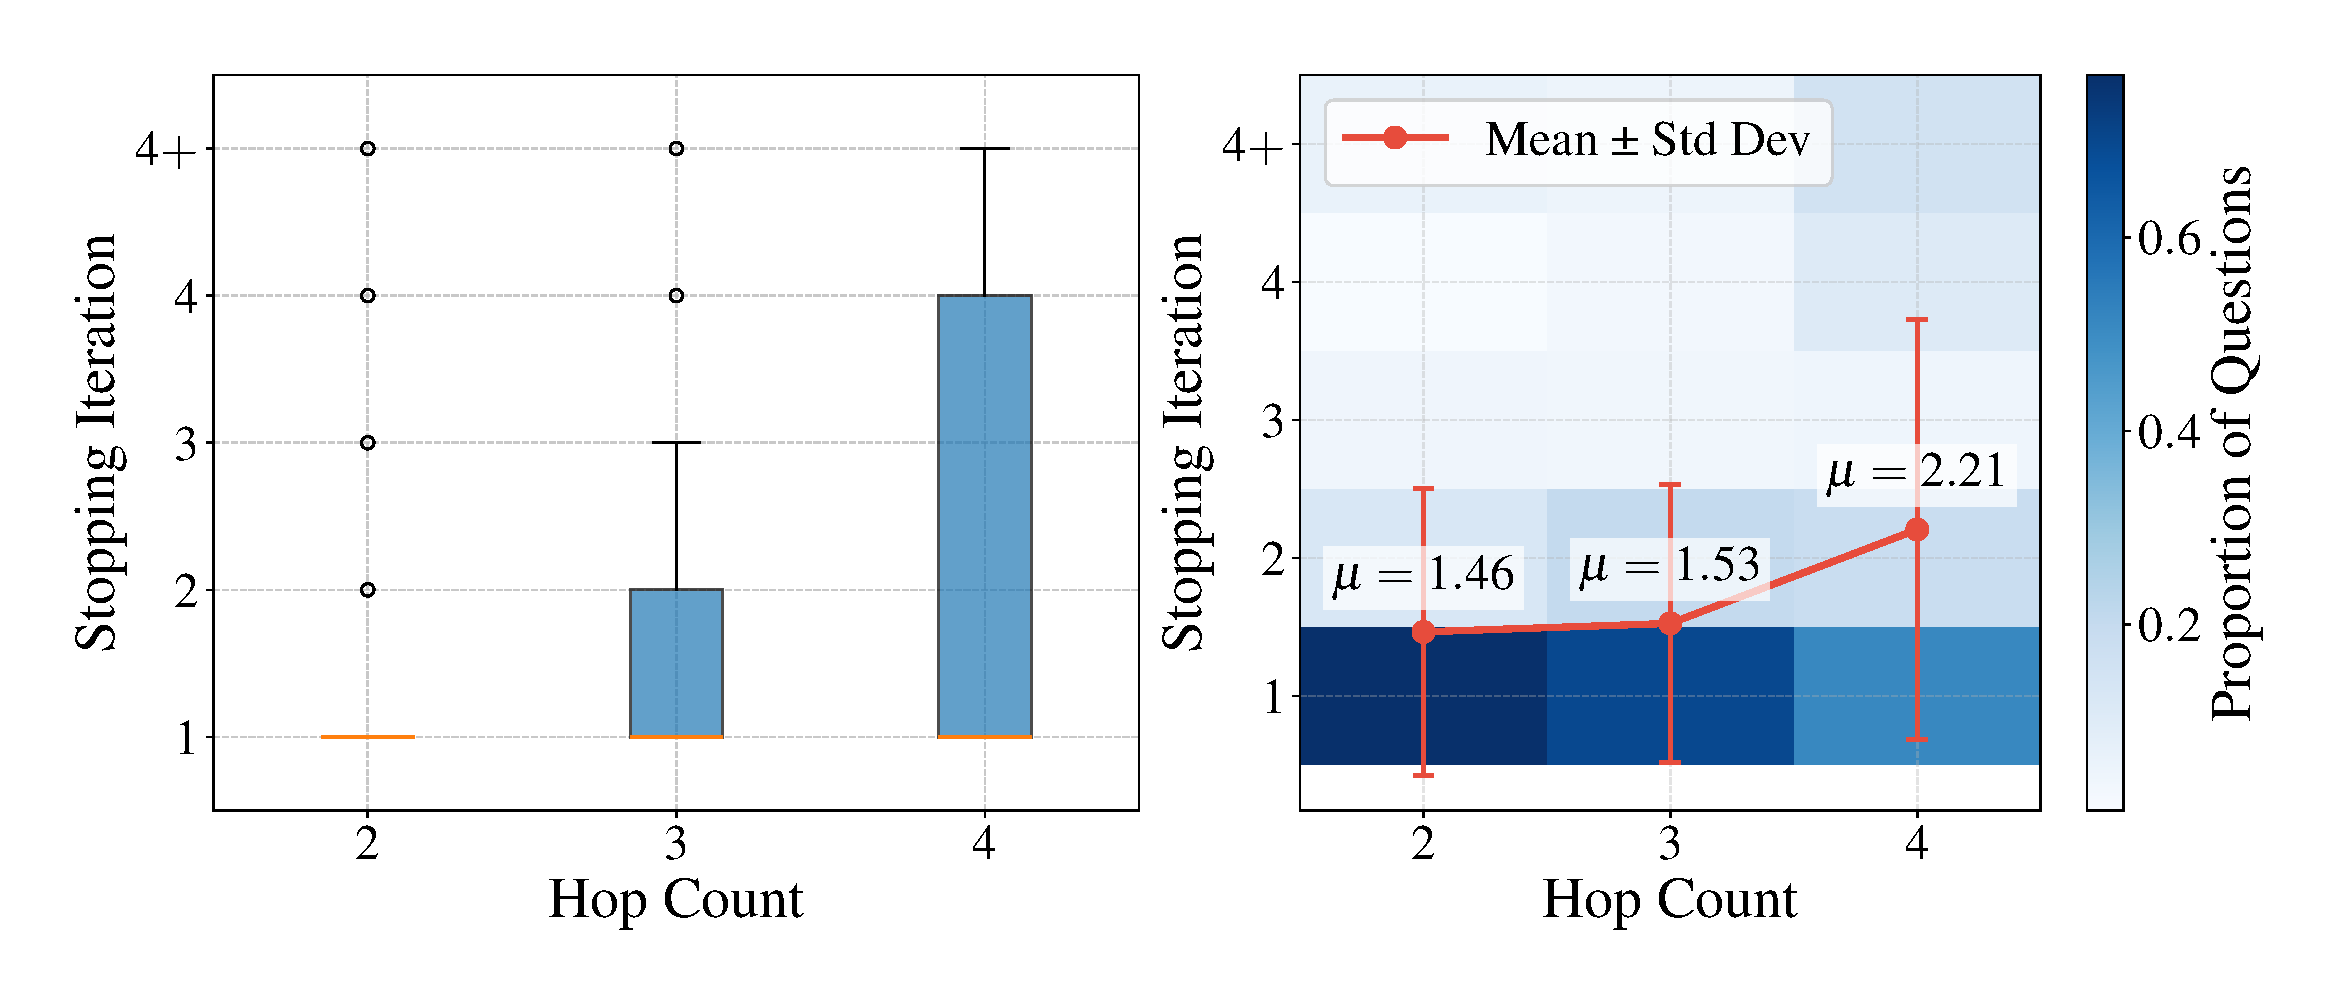
\includegraphics[width=\textwidth]{figures/experiments/hop_vs_agent_iteration_correlation.pdf}
  \caption{Analysis of the relationship between the number of hops in questions and the required number of agent iterations on the MuSiQue dataset. For each hop count, we analyse the number of iterations required by \gear to determine question answerability. The maximum iteration limit was set to 4, with ``4+'' indicating cases where the agent could not determine answerability within this limit. The visualization presents two complementary perspectives on the same data: the left panel shows a box plot emphasizing the median and distribution of stopping iterations, while the right panel focuses on the mean number of iterations across different hop counts.}
  \label{fig:hop_vs_agent_iteration_correlation}
\end{figure*}

The left panel in Figure \ref{fig:hop_vs_agent_iteration_correlation} demonstrates that the median stopping iteration remains consistently at 1 across all hop counts. Additionally, the upper quartile shows a clear upward trend as the number of hops increases. This suggests greater variability in processing time for more complex questions. The right panel illustrates two concurrent trends: as the question hop count increases, the number of questions in the dataset decreases, and the mean number of iterations \gear requires to determine question answerability increases. This pattern indicates that higher-hop questions not only appear less frequently but also typically demand more computational effort to process.

\section{Qualitative Analysis}
\label{appendix_sec:qualitative_analysis}

\begin{table*}[!thbp]
\centering
\small
\begin{tabular}{@{}L{3.5cm}L{7.3cm}L{4cm}@{}}
\toprule
\rowcolor{white} % Example coloring for header row
\textbf{Query} & \textbf{\gear} & \textbf{HippoRAG w$/$ IRCoT} \\
\midrule

% First row
\cellcolor{white}\begin{tabular}[l]{@{}l@{}}What team is the player who\\ led the league in sacks in\\ 2017 a member of?\end{tabular} & 
\cellcolor{customGreen}\begin{tabular}[c]{@{}l@{}}("Chandler Jones", "team",\ "Arizona Cardinals")\\ ("Chandler Jones", "led the\ league in sacks in", "2017")\end{tabular} & 
\cellcolor{customRed}To answer the question about the player who led the league in sacks in 2017, I need to identify the player and their team from external sources, as the provided documents do not contain that specific information \\
\midrule

% Second row
\cellcolor{white}\begin{tabular}[l]{@{}l@{}}Who is the CEO of\\ FleetBoston Financial's\\ purchaser?\end{tabular} & 
\cellcolor{customGreen}\begin{tabular}[c]{@{}l@{}}("FleetBoston Financial",\ "purchaser", "Bank of America")\\ ("Bank of America", "CEO",\ "Brian Moynihan")\end{tabular} & 
\cellcolor{customYellow}The purchaser of FleetBoston Financial is Bank of America. To find the CEO of Bank of America, I need to look for information about the current leadership of the bank. Next, I will check for the current CEO of Bank of America to answer the question accurately.\\
\midrule

% Third row
\cellcolor{white}\begin{tabular}[l]{@{}l@{}}What UK label was purchased\\ by the company that, along\\ with the distributor of The\\ Cube, and ABC, is the other\\ major New York-based\\ broadcaster?\end{tabular} & 
\cellcolor{customGreen}\begin{tabular}[c]{@{}l@{}}("CBS", "purchased",\ "Oriole Records")\\ ("CBS", "is a major broadcaster\ based in", "New York")\\ ("NBC", "is a major broadcaster\ based in", "New York")\\ ("The Cube", "was distributed\ by", "NBC")\end{tabular} & 
\cellcolor{customYellow}The original network of Undercovers is NBC, which is one of the major broadcasters based in New York. Now, I need to find out which UK label was bought by NBC ... \\
\midrule

% Fourth row
\cellcolor{white}\begin{tabular}[l]{@{}l@{}}What was the 2018\\ population of the Italian\\ city that's underwater?\end{tabular} & 
\cellcolor{customGreen}\begin{tabular}[c]{@{}l@{}}("Venice", "population in 2018",\ "260,897")\end{tabular} & 
\cellcolor{customRed}The Italian city that is underwater is Krag, British Columbia, which is a ghost town... \\
\bottomrule
\end{tabular}
\caption{Comparison of MuSiQue queries where \gear achieves 100\% recall at R@15 in a single iteration, while HippoRAG w$/$ IRCoT shows lower performance despite using all four available iterations. Cell colors indicate recall performance: \colorbox{customGreen}{green} for 100\% recall, \colorbox{customRed}{red} for 0\% recall, and \colorbox{customYellow}{yellow} for any intermediate value. Cell values in \gear represent the proximal triples stored in the Gist Triple Memory. Cell values in HippoRAG w$/$ IRCoT represent IRCoT's thought process.}
\label{tab:triple_extraction_comparison}
\end{table*}


Table \ref{tab:triple_extraction_comparison} showcases some query instances where \gear achieves perfect recall in a single iteration, while HippoRAG w$/$ IRCoT achieves lower recall and consumes all available iterations. The presented examples illustrate how \gear's Gist Memory $\mathcal{G}^{(n)}$ precisely captures the essential information needed to answer MuSiQue's queries, maintaining the appropriate level of granularity without including superfluous details. In contrast, HippoRAG w/ IRCoT struggles to retrieve crucial information—whether due to limitations in its triple extraction step or retriever functionality—such as the exact population of Venice, which is necessary for accurate responses. Furthermore, the verbose nature of IRCoT's thought process component contrasts with \gear's streamlined approach. The lack of such verbose component in our approach contributes to the fact that \gear requires fewer LLM tokens than the competition, as explained in subsection \ref{subsec:gear_efficient}. 

\section{Increasing Number of Agent Iterations}
\label{appendix_sec:increasing_n_iterations}
\begin{figure*}[thbp]
\centering
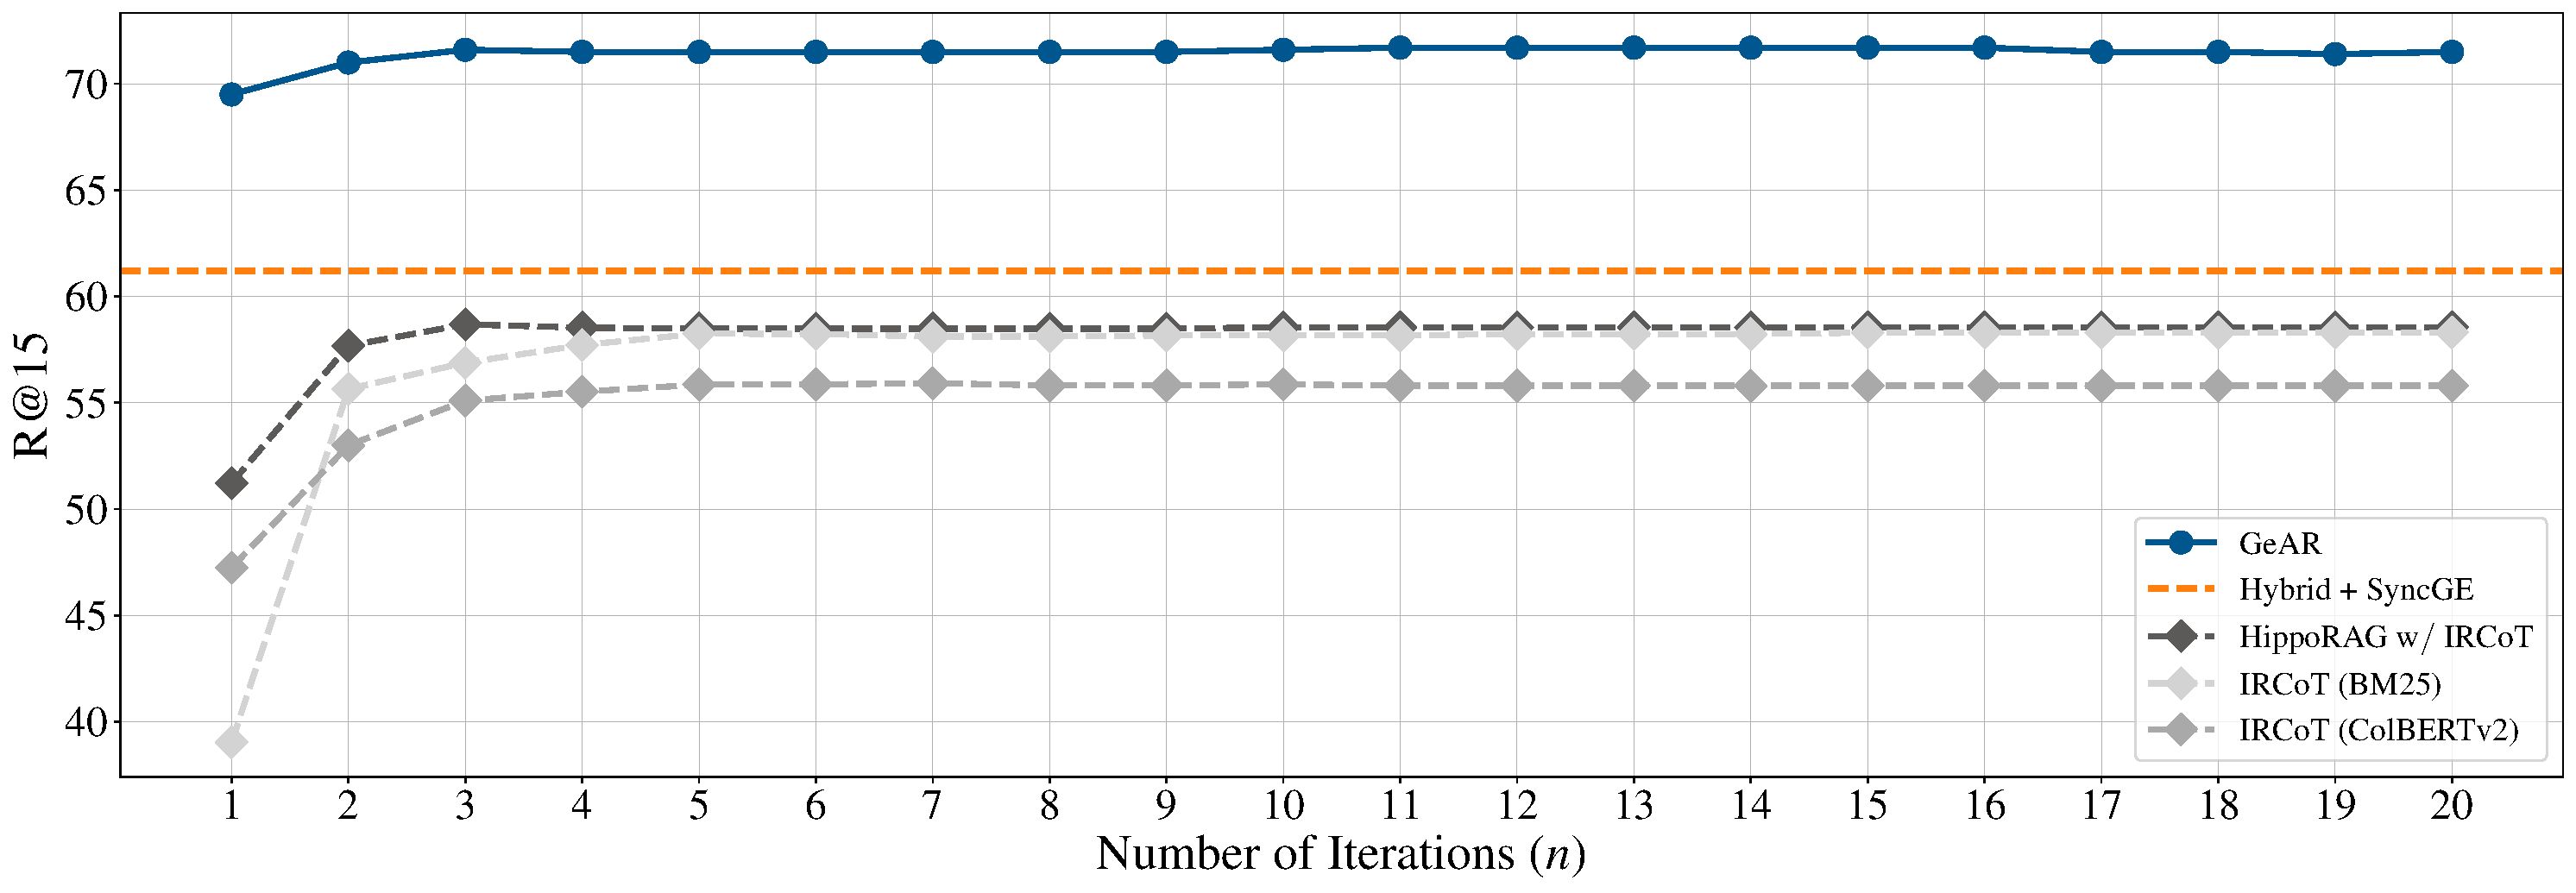
\includegraphics[width=\textwidth]{figures/experiments/recall_evolution_across_agent_iterations_20_iters.pdf}
\caption{Evolution of R@15 over 20 iterations on MuSiQue. Recall is computed at each iteration using the cumulative set of retrieved documents, with prior recall values carried forward for questions that terminated in earlier iterations. The horizontal line indicates the single-step performance of Hybrid + SyncGE.}
\label{fig:recall_across_iterations_20_iters}
\end{figure*}

Figure \ref{fig:recall_across_iterations_20_iters} expands upon the analysis shown in Figure \ref{fig:recall_across_iterations} by evaluating retrieval performance over 20 iterations, rather than the initial 4 iterations. The results demonstrate a consistent pattern across all methods: retrieval performance stabilises after approximately 4 iterations, with no substantial improvements or degradation in subsequent iterations. While some minor fluctuations occur beyond this point, they are negligible.

This performance plateau can be attributed to two key factors. First, the query re-writing mechanisms in all investigated approaches struggle to generate effective subsequent queries. Second, our analysis has identified several cases of unanswerable queries within MuSiQue's answerable subset. A representative example is provided in Table~\ref{tab:musique_problematic_example}.


\begin{table*}
\centering
\footnotesize
\begin{tabular}{L{3cm}L{12cm}}

\toprule
\textbf{Question} & Who did the \textcolor{red}{producer} of \textcolor{purple}{Big Jim McLain} play in \textcolor{purple}{True Grit}? \\
\midrule
\multirow{3.5}{*}{\textbf{Gold Passages}} & {1. \textcolor{purple}{Big Jim McLain}: \textcolor{purple}{Big Jim McLain} is a 1952 political thriller film starring John Wayne and James Arness as HUAC investigators.}\\\cmidrule{2-2}
& {2. \textcolor{purple}{True Grit} is a 1969 American western film. It is the first film adaptation of Charles Portis' 1968 novel of the same name. The screenplay was written by Marguerite Roberts. The film was directed by Henry Hathaway and starred Kim Darby as Mattie Ross and John Wayne as U.S. Marshal Rooster Cogburn. Wayne won his only Academy Award for his performance in this film and reprised his role for the 1975 sequel Rooster Cogburn.}\\
\midrule
\textbf{Comment} & \textcolor{red}{No information about who was the producer of} \textcolor{purple}{Big Jim McLain} \textcolor{red}{is provided in the gold passages}\\
\bottomrule
\end{tabular}
\caption{\label{tab:musique_problematic_example}Example of a query from MuSiQue that in not answerable solely based on the provided gold passages.}
\end{table*}

\section{Comparison of Triple Extraction Prompting Strategies}
\label{appendix_sec:hipporag_results_original_prompt}

\begin{table*}[thbp]
\small
\centering
\resizebox{\textwidth}{!}{%
\begin{tabular}{l l ccc ccc ccc}
\toprule
& & \multicolumn{3}{c}{\textbf{MuSiQue}} & \multicolumn{3}{c}{\textbf{2Wiki}} & \multicolumn{3}{c}{\textbf{HotpotQA}} \\ 
\cmidrule(lr){3-5} \cmidrule(lr){6-8} \cmidrule(lr){9-11}
& & R@5 & R@10 & R@15 & R@5 & R@10 & R@15 & R@5 & R@10 & R@15 \\ 
\midrule
\multirow{2}{*}{\parbox[t]{4cm}{\textbf{HippoRAG}}}
& original prompt & \textbf{41.9} & 46.9 & 51.1 & \textbf{75.4} & \textbf{83.5} & \textbf{86.9} & 79.7 & 88.4 & 91.4 \\ 
& our prompt & 41.0 & \textbf{47.0} & \textbf{51.4} & 75.1 & 83.2 & 86.4 & \textbf{79.8} & \textbf{89.0} & \textbf{92.4} \\ 
\midrule
\multirow{2}{*}{\parbox[t]{4cm}{\textbf{HippoRAG w/ IRCoT}}}
& original prompt & \textbf{49.9} & \textbf{56.4} & \textbf{59.3} & 81.5 & 90.2 & 92.3 & \textbf{90.2} & \textbf{94.7} & 95.8 \\ 
& our prompt & 48.8 & 54.5 & 58.9 & \textbf{82.9} & \textbf{90.6} & \textbf{93.0} & 90.1 & \textbf{94.7} & \textbf{95.9} \\ 
\bottomrule
\end{tabular}}
\caption{Retrieval performance comparison between HippoRAG's sequential triple extraction method and our joint extraction approach across three datasets.}
\label{tab:hippo_prompt_vs_our_prompt}
\end{table*}

HippoRAG employs a sequential approach to triple extraction: it first identifies named entities from a text chunk, and then uses these entities to guide triple extraction in a second step. In contrast, our method extracts both entities and triples simultaneously. Table \ref{tab:hippo_prompt_vs_our_prompt} shows that both approaches achieve comparable retrieval performance across all datasets, with each method excelling in different scenarios. These results validate that joint entity and triple extraction can match the effectiveness of sequential extraction while reducing the number of required processing steps.

\clearpage
\onecolumn  % Switch to one column before strip environment
\section{Prompts}
\label{appendix_sec:agent_prompts}

\subsection{Offline Prompts}
\label{sec:offline_prompts}
\begin{prompt}[title={Reader}]
 \textbf{\# Instruction} \\
\\
Your task is to construct an RDF (Resource Description Framework) graph from the given passages and named entity lists. \\
Respond with a JSON list of triples, with each triple representing a relationship in the RDF graph. \\
Pay attention to the following requirements: \\
- Each triple should contain at least one, but preferably two, of the named entities in the list for each passage. \\
- Clearly resolve pronouns to their specific names to maintain clarity. \\
\\
Convert the paragraph into a JSON dict containing a named entity list and a triple list. \\
\\
\ \textbf{\# Demonstration \#1} \\
\\
Paragraph: \\
``` \\
Magic Johnson \\
\\
After winning a national championship with Michigan State in 1979, Johnson was selected first overall in the 1979 NBA draft by the Lakers, leading the team to five NBA championships during their "Showtime" era. \\
``` \\
\{\{"named\_entities": ["Michigan State", "national championship", "1979", "Magic Johnson", \\ "National Basketball Association", "Los Angeles Lakers", "NBA Championship"]\}\} \\
\{\{ \\
    "triples": [ \\
        ("Magic Johnson", "member of sports team", "Michigan State"), \\
        ("Michigan State", "award", "national championship"), \\
        ("Michigan State", "award date", "1979"), \\
        ("Magic Johnson", "draft pick number", "1"), \\
        ("Magic Johnson", "drafted in", "1979"), \\
        ("Magic Johnson", "drafted by", "Los Angeles Lakers"), \\
        ("Magic Johnson", "member of sports team", "Los Angeles Lakers"), \\
        ("Magic Johnson", "league", "National Basketball Association"), \\
        ("Los Angeles Lakers", "league", "National Basketball Association"), \\
        ("Los Angeles Lakers", "award received", "NBA Championship"), \\
    ] \\
\}\} \\
``` \\
\\
\ \textbf{\# Demonstration \#2} \\
\\
Paragraph: \\
``` \\
Elden Ring \\
\\
Elden Ring is a 2022 action role-playing game developed by FromSoftware. It was directed by Hidetaka Miyazaki with worldbuilding provided by American fantasy writer George R. R. Martin. \\
``` \\
\{\{"named\_entities": ["Elden Ring", "2022", "Role-playing video game", "FromSoftware", "Hidetaka Miyazaki", "United States of America", "fantasy", "George R. R. Martin"]\}\} \\
\{\{ \\
    "triples": [ \\
        ("Elden Ring", "publication", "2022"), \\
        ("Elden Ring", "genre", "action role-playing game"), \\
        ("Elden Ring", "publisher", "FromSoftware"), \\
        ("Elden Ring", "director", "Hidetaka Miyazaki"), \\
        ("Elden Ring", "screenwriter", "George R. R. Martin"), \\
        ("George R. R. Martin", "country of citizenship", "United States of America"), \\
        ("George R. R. Martin", "genre", "fantasy"), \\
    ] \\
\}\} \\
\\
\\
\ \textbf{\# Input} \\
\\
Convert the paragraph into a JSON dict, it has a named entity list and a triple list. \\
\\
Paragraph: \\
``` \\
\textbf{$\{$wiki\_title$\}$} \\
\\
\textbf{$\{$passage$\}$}\\
\end{prompt}

\subsection{Online Retrieval Prompts}
\label{subsec:online_retrieval_prompts}

The \textcolor{blue}{blue}-highlighted portions of the Reader prompt below indicate additional text that is only required when the Gist Memory $\mathcal{G}^{(n)}$ is active. When Gist Memory is inactive, these blue sections should be omitted, and the $\{$triples$\}$ parameter should be left empty.

\begin{prompt}[title={Reader with and without Gist Memory }]
Your task is to find facts that help answer an input question. \\
\\
You should present these facts as knowlege triples, which are structured as ("subject", "predicate", "object"). \\
Example: \\
Question: When was Neville A. Stanton's employer founded? \\
Facts: ("Neville A. Stanton", "employer", "University of Southampton"), ("University of Southampton", "founded in", "1862") \\
\\
\\
Now you are given some documents:\\
\textbf{$\{$docs$\}$} \\
\\
\\
Based on these documents \textcolor{blue}{and some preliminary facts provided below}, \\ find additional supporting fact(s) that may help answer the following question. \\
 \\
Note: if the information you are given is insufficient, output only the relevant facts you can find.\\
\\
Question: \textbf{$\{$query$\}$} \\
Facts: \textcolor{blue}{\textbf{$\{$triples$\}$}} \\
\end{prompt}

\begin{prompt}[title={Reasoning for Termination}]
\ \textbf{\# Task Description:} \\
You are given an input question and a set of known facts:\\
Question: \textbf{$\{$query$\}$} \\
Facts: \textbf{$\{$triples$\}$} \\
\\
Your reply must follow the required format:\\
1. If the provided facts contain the answer to the question, your should reply as follows:\\
Answerable: Yes\\
Answer: ...\\
\\
2. If not, you should explain why and reply as follows:\\
Answerable: No\\
Why: ...\\
\\
\ \textbf{\# Your reply:} \\
\end{prompt}


\begin{prompt}[title={Query Re-writing}]
\ \textbf{\# Task Description:} \\
You will be presented with an input question and a set of known facts. \\
These facts might be insufficient for answering the question for some reason. \\
Your task is to analyze the question given the provided facts and 
determine what else information is needed for the next step. \\
\\
\ \textbf{\# Example:} \\
Question: What region of the state where Guy Shepherdson was born, contains SMA Negeri 68?\\
Facts: ("Guy Shepherdson", "born in", "Jakarta")\\
Reason: The provided facts only indicate that Guy Shepherdson was born in Jakarta, but they do not provide any information about the region of the state that contains SMA Negeri 68. \\
Next Question: What region of Jakarta contains SMA Negeri 68? \\
\\
\ \textbf{\# Your Task:} \\
Question: \textbf{$\{$query$\}$} \\
Facts: \textbf{$\{$triples$\}$} \\
Reason: \textbf{$\{$reason$\}$} \\
\\
Next Question:
\end{prompt}

\subsection{Online Question Answering Prompts}

The following prompt with retrieved passages combines the QA generation prompts from \citeauthor{Gutierrez2024} and \citeauthor{Wang2024}. For the variation without retrieved passages, we omit the preamble and only include the instruction, highlighted in \textcolor{purple}{purple} .

\begin{prompt}[title={Retrieved Passages with In-context Example}]
As an advanced reading comprehension assistant, your task is to analyze text passages and corresponding questions meticulously, with the aim of providing the correct answer. \\
==================\\
For example:\\
==================\\
Wikipedia Title: Edward L. Cahn \\
Edward L. Cahn (February 12, 1899 – August 25, 1963) was an American film director.\\
\\
Wikipedia Title: Laughter in Hell \\
Laughter in Hell is a 1933 American Pre-Code drama film directed by Edward L. Cahn and starring Pat O'Brien. The film's title was typical of the sensationalistic titles of many Pre-Code films. Adapted from the 1932 novel of the same name buy Jim Tully, the film was inspired in part by "I Am a Fugitive from a Chain Gang" and was part of a series of films depicting men in chain gangs following the success of that film. O'Brien plays a railroad engineer who kills his wife and her lover in a jealous rage and is sent to prison. The movie received a mixed review in "The New York Times" upon its release. Although long considered lost, the film was recently preserved and was screened at the American Cinematheque in Hollywood, CA in October 2012. The dead man's brother ends up being the warden of the prison and subjects O'Brien's character to significant abuse. O'Brien and several other characters revolt, killing the warden and escaping from the prison. The film drew controversy for its lynching scene where several black men were hanged. Contrary to reports, only blacks were hung in this scene, though the actual executions occurred off-camera (we see instead reaction shots of the guards and other prisoners). The "New Age" (an African American weekly newspaper) film critic praised the scene for being courageous enough to depict the atrocities that were occurring in some southern states. \\
\\
Wikipedia Title: Theodred II (Bishop of Elmham) \\
Theodred II was a medieval Bishop of Elmham. The date of Theodred's consecration unknown, but the date of his death was sometime between 995 and 997. \\
\\
Wikipedia Title: Etan Boritzer \\
Etan Boritzer( born 1950) is an American writer of children 's literature who is best known for his book" What is God?" first published in 1989. His best selling" What is?" illustrated children's book series on character education and difficult subjects for children is a popular teaching guide for parents, teachers and child- life professionals. Boritzer gained national critical acclaim after" What is God?" was published in 1989 although the book has caused controversy from religious fundamentalists for its universalist views. The other current books in the" What is?" series include What is Love?, What is Death?, What is Beautiful?, What is Funny?, What is Right?, What is Peace?, What is Money?, What is Dreaming?, What is a Friend?, What is True?, What is a Family?, What is a Feeling?" The series is now also translated into 15 languages. Boritzer was first published in 1963 at the age of 13 when he wrote an essay in his English class at Wade Junior High School in the Bronx, New York on the assassination of John F. Kennedy. His essay was included in a special anthology by New York City public school children compiled and published by the New York City Department of Education. \\
\\
Wikipedia Title: Peter Levin \\
Peter Levin is an American director of film, television and theatre. \\
\\
Question: When did the director of film Laughter In Hell die? \\
Answer: August 25, 1963. \\
================== \\
\textcolor{purple}{Given the following text passages and questions, please present a concise, definitive answer, devoid of additional elaborations, and of maximum length of 6 words.} \\
================== \\
\\
Wikipedia Title : \textbf{$\{$title$\}$}
\textbf{$\{$text$\}$} \texttt{for each retrieved passage} ...  \\
Question: \textbf{$\{$question$\}$} \\
\\
Answer:
\end{prompt}

\label{subsec:online_qa_prompts}
\begin{prompt}[title={No Retrieved Passages}]
\textcolor{purple}{Given the following question, please present a concise, definitive answer, devoid of additional elaborations, and of maximum length of 6 words.} \\
\\
Question: \textbf{$\{$question$\}$} \\
\\
Answer:
\end{prompt}


\end{document}
